\documentclass[aspectratio=169,11pt]{beamer}
% ==========================================================================
%  KSA lecture-slide theme  =  stock beamer "Boadilla"  +  KSA colour theme
%  brand colours sampled from the official KSA symbol mark:
%    Deep Prussian Blue  #2E3192   (지성 - intellect)
%    Golden Gray         #D6CBB1   (감성 - sensibility)
%  Engine: XeLaTeX.  Usage:
%    \documentclass[aspectratio=169,11pt]{beamer}
%    % ==========================================================================
%  KSA lecture-slide theme  =  stock beamer "Boadilla"  +  KSA colour theme
%  brand colours sampled from the official KSA symbol mark:
%    Deep Prussian Blue  #2E3192   (지성 - intellect)
%    Golden Gray         #D6CBB1   (감성 - sensibility)
%  Engine: XeLaTeX.  Usage:
%    \documentclass[aspectratio=169,11pt]{beamer}
%    % ==========================================================================
%  KSA lecture-slide theme  =  stock beamer "Boadilla"  +  KSA colour theme
%  brand colours sampled from the official KSA symbol mark:
%    Deep Prussian Blue  #2E3192   (지성 - intellect)
%    Golden Gray         #D6CBB1   (감성 - sensibility)
%  Engine: XeLaTeX.  Usage:
%    \documentclass[aspectratio=169,11pt]{beamer}
%    \input{../theme/ksa-theme.tex}
% ==========================================================================

\usepackage{fontspec}
\usepackage{amsmath,amssymb}
\usepackage{graphicx}
\graphicspath{{figs/}{../figs/}}
\usepackage{booktabs}
\usepackage{listings}

% ---- fonts (no ctex/xeCJK on this box -> fontspec drives CJK directly) -----
\defaultfontfeatures{Ligatures=TeX}
\setmainfont{Noto Sans CJK KR}
\setsansfont{Noto Sans CJK KR}
\setmonofont{Noto Sans Mono CJK KR}[Scale=0.92]

% ---- base theme: stock Boadilla ------------------------------------------
\usetheme{Boadilla}
\usefonttheme{professionalfonts}
\setbeamertemplate{navigation symbols}{}

% ---- KSA colour theme (recolour the stock theme) --------------------------
\definecolor{ksablue}{HTML}{2E3192}
\definecolor{ksabluedk}{HTML}{20226A}
\definecolor{ksagold}{HTML}{D6CBB1}
\definecolor{ksagolddk}{HTML}{A9976B}
\definecolor{ksared}{HTML}{C0392B}
\definecolor{ksagray}{HTML}{5B5B5B}

\setbeamercolor{structure}{fg=ksablue}
\setbeamercolor{alerted text}{fg=ksared}

\setbeamercolor{palette primary}{fg=white,           bg=ksablue}
\setbeamercolor{palette secondary}{fg=white,         bg=ksablue!85!black}
\setbeamercolor{palette tertiary}{fg=white,          bg=ksabluedk}
\setbeamercolor{titlelike}{fg=ksablue}
\setbeamercolor{frametitle}{fg=ksablue,bg=}
\setbeamercolor{title}{fg=ksablue}
\setbeamercolor{author}{fg=ksagray}
\setbeamercolor{institute}{fg=ksagray}
\setbeamercolor{block title}{fg=white,bg=ksablue}
\setbeamercolor{block body}{fg=black!85,bg=ksablue!6}
\setbeamercolor{item}{fg=ksablue}
\setbeamercolor{section in toc}{fg=black!85}

\setbeamerfont{frametitle}{series=\bfseries}
\setbeamerfont{title}{series=\bfseries}

% ---- footline:  KSA mark | "Made by ..." | n / N   (matches reference) ----
\newcommand{\ksacredit}{Made by Sumin Han \,\textperiodcentered\, suminhan@ksa.hs.kr}
\setbeamertemplate{footline}{%
  \hbox{%
    \begin{beamercolorbox}[wd=.18\paperwidth,ht=2.6ex,dp=1.5ex,leftskip=1.1em]{}%
      \raisebox{-0.35ex}{
\includegraphics[height=2.0ex]{ksa-logo.png}}%
    \end{beamercolorbox}%
    \begin{beamercolorbox}[wd=.64\paperwidth,ht=2.6ex,dp=1.5ex,center]{}%
      {\scriptsize\color{ksagray}\ksacredit}%
    \end{beamercolorbox}%
    \begin{beamercolorbox}[wd=.18\paperwidth,ht=2.6ex,dp=1.5ex,rightskip=1.1em]{}%
      \hfill{\scriptsize\color{ksablue}\insertframenumber\,/\,\inserttotalframenumber}%
    \end{beamercolorbox}%
  }%
  \vskip2pt
}

% ---- section divider: stock \sectionpage, KSA-coloured -------------------
\setbeamertemplate{section page}{%
  \begingroup\centering
    {\color{ksagolddk}\rule{0.16\paperwidth}{1pt}}\par\vskip1.0em
    {\usebeamerfont{title}\color{ksablue}\insertsectionhead\par}\vskip1.0em
    {\color{ksagolddk}\rule{0.16\paperwidth}{1pt}}\par
  \endgroup
}
\AtBeginSection[]{\begin{frame}[plain,noframenumbering]\vfill\sectionpage\vfill\end{frame}}

% ---- code listings ------------------------------------------------------------
\lstdefinestyle{ksa}{%
  basicstyle=\ttfamily\scriptsize,
  keywordstyle=\color{ksablue}\bfseries,
  commentstyle=\color{ksagray}\itshape,
  stringstyle=\color{ksagolddk},
  numberstyle=\tiny\color{ksagray},
  backgroundcolor=\color{ksablue!6},
  frame=leftline, framerule=1.4pt, rulecolor=\color{ksablue},
  xleftmargin=1em, aboveskip=0.8em, belowskip=0.4em,
  showstringspaces=false, breaklines=true, language=Python,
}
\lstset{style=ksa}

% ---- handy macros -----------------------------------------------------------
\newcommand{\kb}[1]{\textbf{\color{ksablue}#1}}   % blue keyword
\newcommand{\kq}[1]{\textbf{\color{ksared}#1}}    % red key-question

% ==========================================================================

\usepackage{fontspec}
\usepackage{amsmath,amssymb}
\usepackage{graphicx}
\graphicspath{{figs/}{../figs/}}
\usepackage{booktabs}
\usepackage{listings}

% ---- fonts (no ctex/xeCJK on this box -> fontspec drives CJK directly) -----
\defaultfontfeatures{Ligatures=TeX}
\setmainfont{Noto Sans CJK KR}
\setsansfont{Noto Sans CJK KR}
\setmonofont{Noto Sans Mono CJK KR}[Scale=0.92]

% ---- base theme: stock Boadilla ------------------------------------------
\usetheme{Boadilla}
\usefonttheme{professionalfonts}
\setbeamertemplate{navigation symbols}{}

% ---- KSA colour theme (recolour the stock theme) --------------------------
\definecolor{ksablue}{HTML}{2E3192}
\definecolor{ksabluedk}{HTML}{20226A}
\definecolor{ksagold}{HTML}{D6CBB1}
\definecolor{ksagolddk}{HTML}{A9976B}
\definecolor{ksared}{HTML}{C0392B}
\definecolor{ksagray}{HTML}{5B5B5B}

\setbeamercolor{structure}{fg=ksablue}
\setbeamercolor{alerted text}{fg=ksared}

\setbeamercolor{palette primary}{fg=white,           bg=ksablue}
\setbeamercolor{palette secondary}{fg=white,         bg=ksablue!85!black}
\setbeamercolor{palette tertiary}{fg=white,          bg=ksabluedk}
\setbeamercolor{titlelike}{fg=ksablue}
\setbeamercolor{frametitle}{fg=ksablue,bg=}
\setbeamercolor{title}{fg=ksablue}
\setbeamercolor{author}{fg=ksagray}
\setbeamercolor{institute}{fg=ksagray}
\setbeamercolor{block title}{fg=white,bg=ksablue}
\setbeamercolor{block body}{fg=black!85,bg=ksablue!6}
\setbeamercolor{item}{fg=ksablue}
\setbeamercolor{section in toc}{fg=black!85}

\setbeamerfont{frametitle}{series=\bfseries}
\setbeamerfont{title}{series=\bfseries}

% ---- footline:  KSA mark | "Made by ..." | n / N   (matches reference) ----
\newcommand{\ksacredit}{Made by Sumin Han \,\textperiodcentered\, suminhan@ksa.hs.kr}
\setbeamertemplate{footline}{%
  \hbox{%
    \begin{beamercolorbox}[wd=.18\paperwidth,ht=2.6ex,dp=1.5ex,leftskip=1.1em]{}%
      \raisebox{-0.35ex}{
\includegraphics[height=2.0ex]{ksa-logo.png}}%
    \end{beamercolorbox}%
    \begin{beamercolorbox}[wd=.64\paperwidth,ht=2.6ex,dp=1.5ex,center]{}%
      {\scriptsize\color{ksagray}\ksacredit}%
    \end{beamercolorbox}%
    \begin{beamercolorbox}[wd=.18\paperwidth,ht=2.6ex,dp=1.5ex,rightskip=1.1em]{}%
      \hfill{\scriptsize\color{ksablue}\insertframenumber\,/\,\inserttotalframenumber}%
    \end{beamercolorbox}%
  }%
  \vskip2pt
}

% ---- section divider: stock \sectionpage, KSA-coloured -------------------
\setbeamertemplate{section page}{%
  \begingroup\centering
    {\color{ksagolddk}\rule{0.16\paperwidth}{1pt}}\par\vskip1.0em
    {\usebeamerfont{title}\color{ksablue}\insertsectionhead\par}\vskip1.0em
    {\color{ksagolddk}\rule{0.16\paperwidth}{1pt}}\par
  \endgroup
}
\AtBeginSection[]{\begin{frame}[plain,noframenumbering]\vfill\sectionpage\vfill\end{frame}}

% ---- code listings ------------------------------------------------------------
\lstdefinestyle{ksa}{%
  basicstyle=\ttfamily\scriptsize,
  keywordstyle=\color{ksablue}\bfseries,
  commentstyle=\color{ksagray}\itshape,
  stringstyle=\color{ksagolddk},
  numberstyle=\tiny\color{ksagray},
  backgroundcolor=\color{ksablue!6},
  frame=leftline, framerule=1.4pt, rulecolor=\color{ksablue},
  xleftmargin=1em, aboveskip=0.8em, belowskip=0.4em,
  showstringspaces=false, breaklines=true, language=Python,
}
\lstset{style=ksa}

% ---- handy macros -----------------------------------------------------------
\newcommand{\kb}[1]{\textbf{\color{ksablue}#1}}   % blue keyword
\newcommand{\kq}[1]{\textbf{\color{ksared}#1}}    % red key-question

% ==========================================================================

\usepackage{fontspec}
\usepackage{amsmath,amssymb}
\usepackage{graphicx}
\graphicspath{{figs/}{../figs/}}
\usepackage{booktabs}
\usepackage{listings}

% ---- fonts (no ctex/xeCJK on this box -> fontspec drives CJK directly) -----
\defaultfontfeatures{Ligatures=TeX}
\setmainfont{Noto Sans CJK KR}
\setsansfont{Noto Sans CJK KR}
\setmonofont{Noto Sans Mono CJK KR}[Scale=0.92]

% ---- base theme: stock Boadilla ------------------------------------------
\usetheme{Boadilla}
\usefonttheme{professionalfonts}
\setbeamertemplate{navigation symbols}{}

% ---- KSA colour theme (recolour the stock theme) --------------------------
\definecolor{ksablue}{HTML}{2E3192}
\definecolor{ksabluedk}{HTML}{20226A}
\definecolor{ksagold}{HTML}{D6CBB1}
\definecolor{ksagolddk}{HTML}{A9976B}
\definecolor{ksared}{HTML}{C0392B}
\definecolor{ksagray}{HTML}{5B5B5B}

\setbeamercolor{structure}{fg=ksablue}
\setbeamercolor{alerted text}{fg=ksared}

\setbeamercolor{palette primary}{fg=white,           bg=ksablue}
\setbeamercolor{palette secondary}{fg=white,         bg=ksablue!85!black}
\setbeamercolor{palette tertiary}{fg=white,          bg=ksabluedk}
\setbeamercolor{titlelike}{fg=ksablue}
\setbeamercolor{frametitle}{fg=ksablue,bg=}
\setbeamercolor{title}{fg=ksablue}
\setbeamercolor{author}{fg=ksagray}
\setbeamercolor{institute}{fg=ksagray}
\setbeamercolor{block title}{fg=white,bg=ksablue}
\setbeamercolor{block body}{fg=black!85,bg=ksablue!6}
\setbeamercolor{item}{fg=ksablue}
\setbeamercolor{section in toc}{fg=black!85}

\setbeamerfont{frametitle}{series=\bfseries}
\setbeamerfont{title}{series=\bfseries}

% ---- footline:  KSA mark | "Made by ..." | n / N   (matches reference) ----
\newcommand{\ksacredit}{Made by Sumin Han \,\textperiodcentered\, suminhan@ksa.hs.kr}
\setbeamertemplate{footline}{%
  \hbox{%
    \begin{beamercolorbox}[wd=.18\paperwidth,ht=2.6ex,dp=1.5ex,leftskip=1.1em]{}%
      \raisebox{-0.35ex}{
\includegraphics[height=2.0ex]{ksa-logo.png}}%
    \end{beamercolorbox}%
    \begin{beamercolorbox}[wd=.64\paperwidth,ht=2.6ex,dp=1.5ex,center]{}%
      {\scriptsize\color{ksagray}\ksacredit}%
    \end{beamercolorbox}%
    \begin{beamercolorbox}[wd=.18\paperwidth,ht=2.6ex,dp=1.5ex,rightskip=1.1em]{}%
      \hfill{\scriptsize\color{ksablue}\insertframenumber\,/\,\inserttotalframenumber}%
    \end{beamercolorbox}%
  }%
  \vskip2pt
}

% ---- section divider: stock \sectionpage, KSA-coloured -------------------
\setbeamertemplate{section page}{%
  \begingroup\centering
    {\color{ksagolddk}\rule{0.16\paperwidth}{1pt}}\par\vskip1.0em
    {\usebeamerfont{title}\color{ksablue}\insertsectionhead\par}\vskip1.0em
    {\color{ksagolddk}\rule{0.16\paperwidth}{1pt}}\par
  \endgroup
}
\AtBeginSection[]{\begin{frame}[plain,noframenumbering]\vfill\sectionpage\vfill\end{frame}}

% ---- code listings ------------------------------------------------------------
\lstdefinestyle{ksa}{%
  basicstyle=\ttfamily\scriptsize,
  keywordstyle=\color{ksablue}\bfseries,
  commentstyle=\color{ksagray}\itshape,
  stringstyle=\color{ksagolddk},
  numberstyle=\tiny\color{ksagray},
  backgroundcolor=\color{ksablue!6},
  frame=leftline, framerule=1.4pt, rulecolor=\color{ksablue},
  xleftmargin=1em, aboveskip=0.8em, belowskip=0.4em,
  showstringspaces=false, breaklines=true, language=Python,
}
\lstset{style=ksa}

% ---- handy macros -----------------------------------------------------------
\newcommand{\kb}[1]{\textbf{\color{ksablue}#1}}   % blue keyword
\newcommand{\kq}[1]{\textbf{\color{ksared}#1}}    % red key-question


\title{n-step 부트스트래핑, 적격흔적, 그리고 계획}
\subtitle{n-step TD \,\textperiodcentered\, 적격흔적(TD($\lambda$)) \,\textperiodcentered\, 계획과 학습: Dyna-Q}
\author{Machine Learning 2 \,\textperiodcentered\, 7주차}
\institute{한국과학영재학교 (KSA)}
\date{Chapter 7}

\begin{document}

% ===== title =====
\begin{frame}[plain,noframenumbering]
  \titlepage
\end{frame}

% ===== overview =====
\begin{frame}{이번 주차 개요}
  \begin{itemize}
    \item \kb{7.1 n-step TD: MC와 TD(0) 사이의 다이얼} --- n-step 리턴
      $G_t^{(n)}$을 정의하고, 7-state random walk에서
      $n \in \{1,3,5,10,50\}$으로 30 seed 반복해 U자 곡선을 그린다.
      \texttt{tau = t - n + 1}의 갱신 시차와 할인 지수 오프바이원 버그를
      디버깅한다.
    \item \kb{7.2 적격흔적과 파라미터 튜닝} --- 흔적 $e(s)$로 하나의 TD
      오차가 \textbf{모든 상태를 동시에} 갱신하는 TD($\lambda$)를 배운다.
      ``$\lambda$를 고르는 일''과 ``$n$을 고르는 일''은 같은 U자의 두 모습.
      단 하나의 실행은 믿지 않는다(20회 반복 평균).
    \item \kb{7.3 계획과 학습: Dyna-Q} --- 본 $(s,a)$의 결과 $(r,s')$를
      모델로 저장하고 실제 스텝마다 가상 TD(0) 갱신을 끼워 넣는
      ``경험 $\to$ 학습 $\to$ 모델 저장 $\to$ 계획'' 루프. 5$\times$5 격자에서
      수렴 에피소드 334 $\to$ 35(약 9.5배)의 가속과 한계 효과를 측정한다.
  \end{itemize}
  \vskip0.8em
  \begin{block}{이전·다음과의 연결}
    n-step TD, TD($\lambda$), Dyna-Q는 모두 \textbf{``부트스트래핑을 얼마나
    할 것인가''}라는 하나의 질문에 대한 서로 다른 답. Ch.\,8 캡스톤에서
    Gymnasium의 표 기반 환경으로 세 개를 직접 구현·비교하고,
    n-step 리턴은 Ch.\,9 DQN의 기본 옵션으로 다시 만난다.
  \end{block}
\end{frame}

\section{7.1 n-step TD: MC와 TD(0) 사이의 다이얼}

\begin{frame}{복습: 두 극단 --- MC와 TD(0)}
  \begin{itemize}
    \item MC의 목표값: 에피소드 \textbf{끝까지의} 실제 보상 합(실제 리턴)
      $G_t$ --- 추정치 없음.
    \item TD(0)의 목표값: $r + \gamma V(s')$ --- 실제 보상 $1$개 + 나머지
      추정치.
    \item 나란히 쓰면 \textbf{같은 구조의 다른 길이}: 차이는 ``실제 보상을
      몇 개 쓸 것인가''가 $1$개와 ``끝까지 전부''인 것.
  \end{itemize}
  \vskip0.8em
  \kq{1과 ``끝까지'' 사이의 아무 정수 $n$도 가능해야 하지 않나 ---
  $n$개의 실제 보상 + 나머지는 추정치, 라는 목표값을 쓰자. 이것이
  \kb{n-step TD}.}
\end{frame}

\begin{frame}{n-step 리턴의 정의}
  \begin{block}{n-step 리턴 $G_t^{(n)}$}
    \[
    G_t^{(n)} = R_t + \gamma R_{t+1} + \cdots + \gamma^{n-1} R_{t+n-1}
    + \gamma^n V(s_{t+n})
    \]
  \end{block}
  \begin{itemize}
    \item $n=1$이면 \textbf{정확히 TD(0)}, $n\to\infty$(끝까지)이면
      \textbf{정확히 MC}.
    \item $n$을 늘릴수록 실제 관찰 의존 $\uparrow$ $\Rightarrow$
      \textbf{편향은 줄고 분산은 커진다} (Ch.\,6.1 표의 트레이드오프
      연속선상).
    \item $n$: 그 사이 어딘가를 상황에 맞게 고르는 \kb{하이퍼파라미터}.
  \end{itemize}
\end{frame}

\begin{frame}{세 방법 한눈에 --- 그리고 ``갱신 시차''}
  \small
  \begin{tabular}{@{}lllll@{}}
    \toprule
     & $n$ & 실제 보상 & 추정치(부트스트래핑) & 갱신 \\
    \midrule
    TD(0) & 1 & $R_t$ 1개 & $V(s_{t+1})$ & 매 스텝 즉시 \\
    n-step TD & $n$ & $R_t,\dots,R_{t+n-1}$ $n$개 & $V(s_{t+n})$ & 첫 갱신 $n-1$ 스텝 지연 \\
    MC & $\infty$ & 끝까지 전부 & 없음 & 에피소드 종료 시 \\
    \bottomrule
  \end{tabular}
  \vskip1em
  \begin{block}{기다려야 하는 시간(학습의 시차)}
    $G_t^{(n)}$을 계산하려면 $t$에서 $t+n-1$까지의 보상이 \textbf{다 모여야}
    하므로, $t$번 상태의 \textbf{첫} 갱신은 최소 $n-1$ 스텝 뒤에야
    가능. $n$이 클수록 시차 $\uparrow$.
    \vskip0.3em
    이 시차가 갱신 \textbf{횟수}에는 영향을 주지 않는다(반직관적 ---
    FAQ에서 확인, 실습에서 직접 세어보자).
  \end{block}
\end{frame}

\begin{frame}{환경: 7개 상태 random walk}
  \begin{itemize}
    \item 상태 $0$과 $6$: \textbf{터미널}, $1\sim5$: 이동 상태.
    \item 매 스텝 50:50 좌우 이동(무작위 정책).
    \item 왼쪽 끝 $-1$, 오른쪽 끝 $+1$ 보상. $\gamma = 0.9$,
      상태 $3$에서 시작.
    \item 학습 목표: 이 환경의 \textbf{참값} $V^\pi(s)$와 비교해
      $n$별 추정 품질을 측정.
  \end{itemize}
  \vskip0.8em
  \begin{columns}[T]
    \begin{column}{0.50\textwidth}
      \small
      \begin{tabular}{@{}ll@{}}
        \toprule
        상태 & 참값 $V^\pi$ \\
        \midrule
        0 & 0 (터미널) \\
        1 & $-0.5643$ \\
        2 & $-0.2539$ \\
        3 & 0 (시작, 대칭 중심) \\
        4 & $+0.2539$ \\
        5 & $+0.5643$ \\
        6 & 0 (터미널) \\
        \bottomrule
      \end{tabular}
      {\footnotesize 좌우 미러링(대칭성)으로
      $V(3)=0$, $V(2)=-V(4)$, $V(1)=-V(5)$.}
    \end{column}
    \begin{column}{0.48\textwidth}
      \begin{block}{참값의 모양}
        7-state random walk에서 $n=3$으로 10 에피소드
        ($\alpha=0.1$, seed 고정) 학습하면, 참값의 모양을
        대략 따라가며 \textbf{오른쪽 끝(+1 목표)에 가까울수록
        가치가 매끄럽게 단조 증가}(상태 1 $\approx -0.48$
        에서 오른쪽으로, 상태 5 $\approx +0.37$까지).
        \vskip0.3em
        에피소드가 10개뿐이라 참값까지 다 도달하진 않지만,
        \textbf{방향(오른쪽 > 왼쪽)은 이미 잡혀} 있는 상태.
      \end{block}
    \end{column}
  \end{columns}
\end{frame}

\begin{frame}[fragile]{n-step TD 코드 (1/2)}
  \begin{lstlisting}[basicstyle=\ttfamily\footnotesize]
def n_step_td(env_step, n, n_episodes, alpha, gamma,
              n_states, start_state):
    V = [0.0] * n_states
    for _ in range(n_episodes):
        states, rewards = [start_state], []
        s, T, t = start_state, float('inf'), 0
        while True:
            if t < T:
                a = random.randrange(2)   # 데모용 무작위 정책
                ns, r, done = env_step(s, a)
                states.append(ns); rewards.append(r)
                if done:
                    T = t + 1
                s = ns
            tau = t - n + 1       # tau번 상태를 지금 갱신
            # --- 핵심 3줄은 다음 슬라이드에서 뜯어 봄 ---
            if tau >= 0:
                G = n_step_target(tau)      # 목표값 계산
                V[states[tau]] += alpha * (G - V[states[tau]])
            if tau == T - 1:
                break
            t += 1
    return V
  \end{lstlisting}
  {\footnotesize 환경 \texttt{env\_step}: 0과 6이 터미널,
  \texttt{(next\_state, reward, done)} 반환.}
\end{frame}

\begin{frame}[fragile]{n-step TD 코드 (2/2): 핵심 3줄}
  \begin{lstlisting}[basicstyle=\ttfamily\footnotesize]
            if tau >= 0:
                G = sum(gamma ** (i - tau) * rewards[i]
                        for i in range(tau, min(tau + n, len(rewards))))
                if tau + n < T:
                    G += gamma ** n * V[states[tau + n]]   # 추정치 항
                V[states[tau]] += alpha * (G - V[states[tau]])
  \end{lstlisting}
  \begin{itemize}
    \item $\tau \ge 0$: 실제 보상 $n$개가 다 모인 시점이므로 $G_\tau^{(n)}$
      계산 가능.
    \item \texttt{tau + n < T}: $n$ 스텝 윈도우가 끝나기 \textbf{전에}
      에피소드가 끝나지 않았다면 $\gamma^n V(s_{\tau+n})$을 추가.
      끝나면 \textbf{추정치 항 생략}(절단 목표값).
    \item 이 절단 덕분에 $n$이 에피소드 길이보다 길면 \textbf{자동으로
      MC}가 됨 --- $n=50$이 사실상 MC로 동작하는 이유(이 환경 에피소드
      길이는 보통 50보다 짧음).
  \end{itemize}
\end{frame}

\begin{frame}{왜 $\tau = t - n + 1$인가 --- 갱신 시차}
  \begin{itemize}
    \item $\tau$(갱신 대상 시점)는 항상 현재 $t$보다 \textbf{$n-1$만큼
      뒤처짐} --- $n$ 스텝의 실제 보상이 다 모여야 목표값을 계산
      가능.
    \item $t$가 한 스텝씩 가면 갱신 차례인 $\tau$도 한 칸씩 앞으로
      밀려남.
    \item 에피소드 종료(``$t \ge T$'') 이후에도 이 밀림이
      \texttt{tau == T-1}까지 계속됨 --- 아직 $n$ 스텝 목표값을
      계산 못 한 상태가 남아 있어서(꼬리 갱신).
  \end{itemize}
  \vskip0.8em
  \begin{block}{갱신 횟수는 변하지 않는다}
    에피소드가 $T$ 이동 상태면 $n=1$이든 $n=T+1$이든 \textbf{모든
    이동 상태마다 정확히 1번씩}(총 $T$번) 갱신된다. $n$이 바꾸는
    것은 갱신 \textbf{횟수}가 아니라, 첫 갱신까지의 \textbf{시차}와
    목표값의 \textbf{구성}(실제/추정 비율).
  \end{block}
\end{frame}

\begin{frame}[fragile]{중요: 목표값의 할인 지수를 세어라}
  \begin{itemize}
    \item $G_t^{(n)}$ 정의에서 $R_{t+k}$의 지수는 $k$. $\tau$번 상태
      갱신 시: \texttt{rewards[tau]} 지수 $0$, \texttt{rewards[tau+1]}
      지수 $1$, …, \texttt{rewards[i]}의 지수는 $\mathbf{i - \tau}$.
    \item 여기서 \textbf{하나만} 틀리면:
  \end{itemize}
  \begin{lstlisting}[basicstyle=\ttfamily\footnotesize]
    G = sum(gamma ** (i - tau - 1) * rewards[i] for i in ...)
    # 각 보상이 gamma^{-1}만큼 "덜" 할인된 -> 편향된 목표값
  \end{lstlisting}
  \begin{itemize}
    \item 이렇게 쓰면 $n=1$일 때조차 \textbf{TD(0)의 목표값이 아님}.
      2000 에피소드 학습 후에도 $V(5) \approx 0.84$로 참값
      $+0.5643$에서 크게 벗어나 \textbf{수렴하지 않음}.
    \item 지수 하나가 틀리면 ``TD(0)를 쓰는 것''이 아니라
      \textbf{``편향된 목표값을 끝없이 쓰는 것''}.
  \end{itemize}
\end{frame}

\begin{frame}{online 관점 vs forward 관점}
  \begin{columns}[T]
    \begin{column}{0.49\textwidth}
      \kb{online 관점 (online view)}
      \begin{itemize}
        \item 학습이 \textbf{진행되면서} 목표를 만들어 갱신.
        \item ``지금 $t$ 스텝을 왔다'' $\to$ 지금까지 \textbf{실제로
          쌓인} $R_t,\dots,R_{t+n-1}$으로 $G_t^{(n)}$ 계산.
        \item 위 코드의 \texttt{tau = t - n + 1}과 \texttt{tau + n < T}
          분기가 바로 산물.
        \item 실제 알고리즘의 \textbf{실행 순서}(갱신 시차, 에피소드
          끝 처리)를 정확히 반영.
      \end{itemize}
    \end{column}
    \begin{column}{0.49\textwidth}
      \kb{forward 관점 (forward view)}
      \begin{itemize}
        \item 같은 경험(trajectory) 위에서 $n$을 바꾸면
          \textbf{서로 다른 목표값}이 생김.
        \item $n=1$: $R_t + \gamma V(s_{t+1})$
        \item $n=2$: $R_t + \gamma R_{t+1} + \gamma^2 V(s_{t+2})$
        \item ``$n$이 커지면 MC에 가까워진다''는 직관(목표값
          \textbf{정의 자체}에서 $n\to\infty$가 MC 리턴)을 가장
          투명하게 보여줌.
      \end{itemize}
    \end{column}
  \end{columns}
  \vskip0.6em
  {\footnotesize 두 관점은 \textbf{동일한 알고리즘}을 기술. 7.2의
  적격흔적은 ``모든 $n$을 동시에'' 쓰면서 이 연결의 핵심이 됨.}
\end{frame}

\begin{frame}{왜 $n$이 커지면 편향은 줄고 분산은 커지는가}
  \begin{itemize}
    \item $V$가 참값 $V^\pi$라면 $G_t^{(n)}$의 기대값은
      \textbf{정확히} $V^\pi(s_t)$ --- 실제 보상 합이 ``앞으로 받을
      할인 보상의 기댓값''의 단일 샘플(모든 $n$에서 성립).
    \item 학습 초반 $V \ne V^\pi$: 목표값에 추정치가 \textbf{일부}
      섞여 있는 것 = \kb{편향(bias)}의 출처.
  \end{itemize}
  \begin{columns}[T]
    \begin{column}{0.49\textwidth}
      \kb{편향 $\downarrow$}
      $n$이 커지면 목표에서 추정치 비중 $\downarrow$, 실제 보상
      비중 $\uparrow$ $\Rightarrow$ $V$가 부정확해도 목표값이 참값에
      가까워짐.
    \end{column}
    \begin{column}{0.49\textwidth}
      \kb{분산 $\uparrow$}
      실제 보상 합이 길어지면 각 스텝의 전이·보상 무작위성이 더 많이
      누적됨. MC가 ``분산 극대''인 이유와 정확히 같음.
    \end{column}
  \end{columns}
  \vskip0.6em
  {\footnotesize ML1 Ch.\,4.1의 \textbf{편향-분산 트레이드오프}가 여기서는
  $n$이라는 하나의 다이얼 위 숫자로 드러남.}
\end{frame}

\begin{frame}{U자 곡선: n별 RMS 오차 (30 seed 평균)}
  \begin{columns}[T]
    \begin{column}{0.45\textwidth}
      \small
      \begin{tabular}{@{}ll@{}}
        \toprule
        $n$ & RMS 오차 (10 에피소드) \\
        \midrule
        1 (TD(0)) & 0.4007 \\
        \textbf{3} & \textbf{0.3061} $\leftarrow$ 이 환경·예산에서 최적 \\
        5 & 0.3493 \\
        10 & 0.3994 \\
        50 (사실상 MC) & 0.4170 \\
        \bottomrule
      \end{tabular}
      \vskip0.6em
      설정: $\alpha=0.1$, $\gamma=0.9$, 10 에피소드, 30 seed.
      오차가 $n$에 대해 \textbf{U자}.
    \end{column}
    \begin{column}{0.53\textwidth}
      \centering
      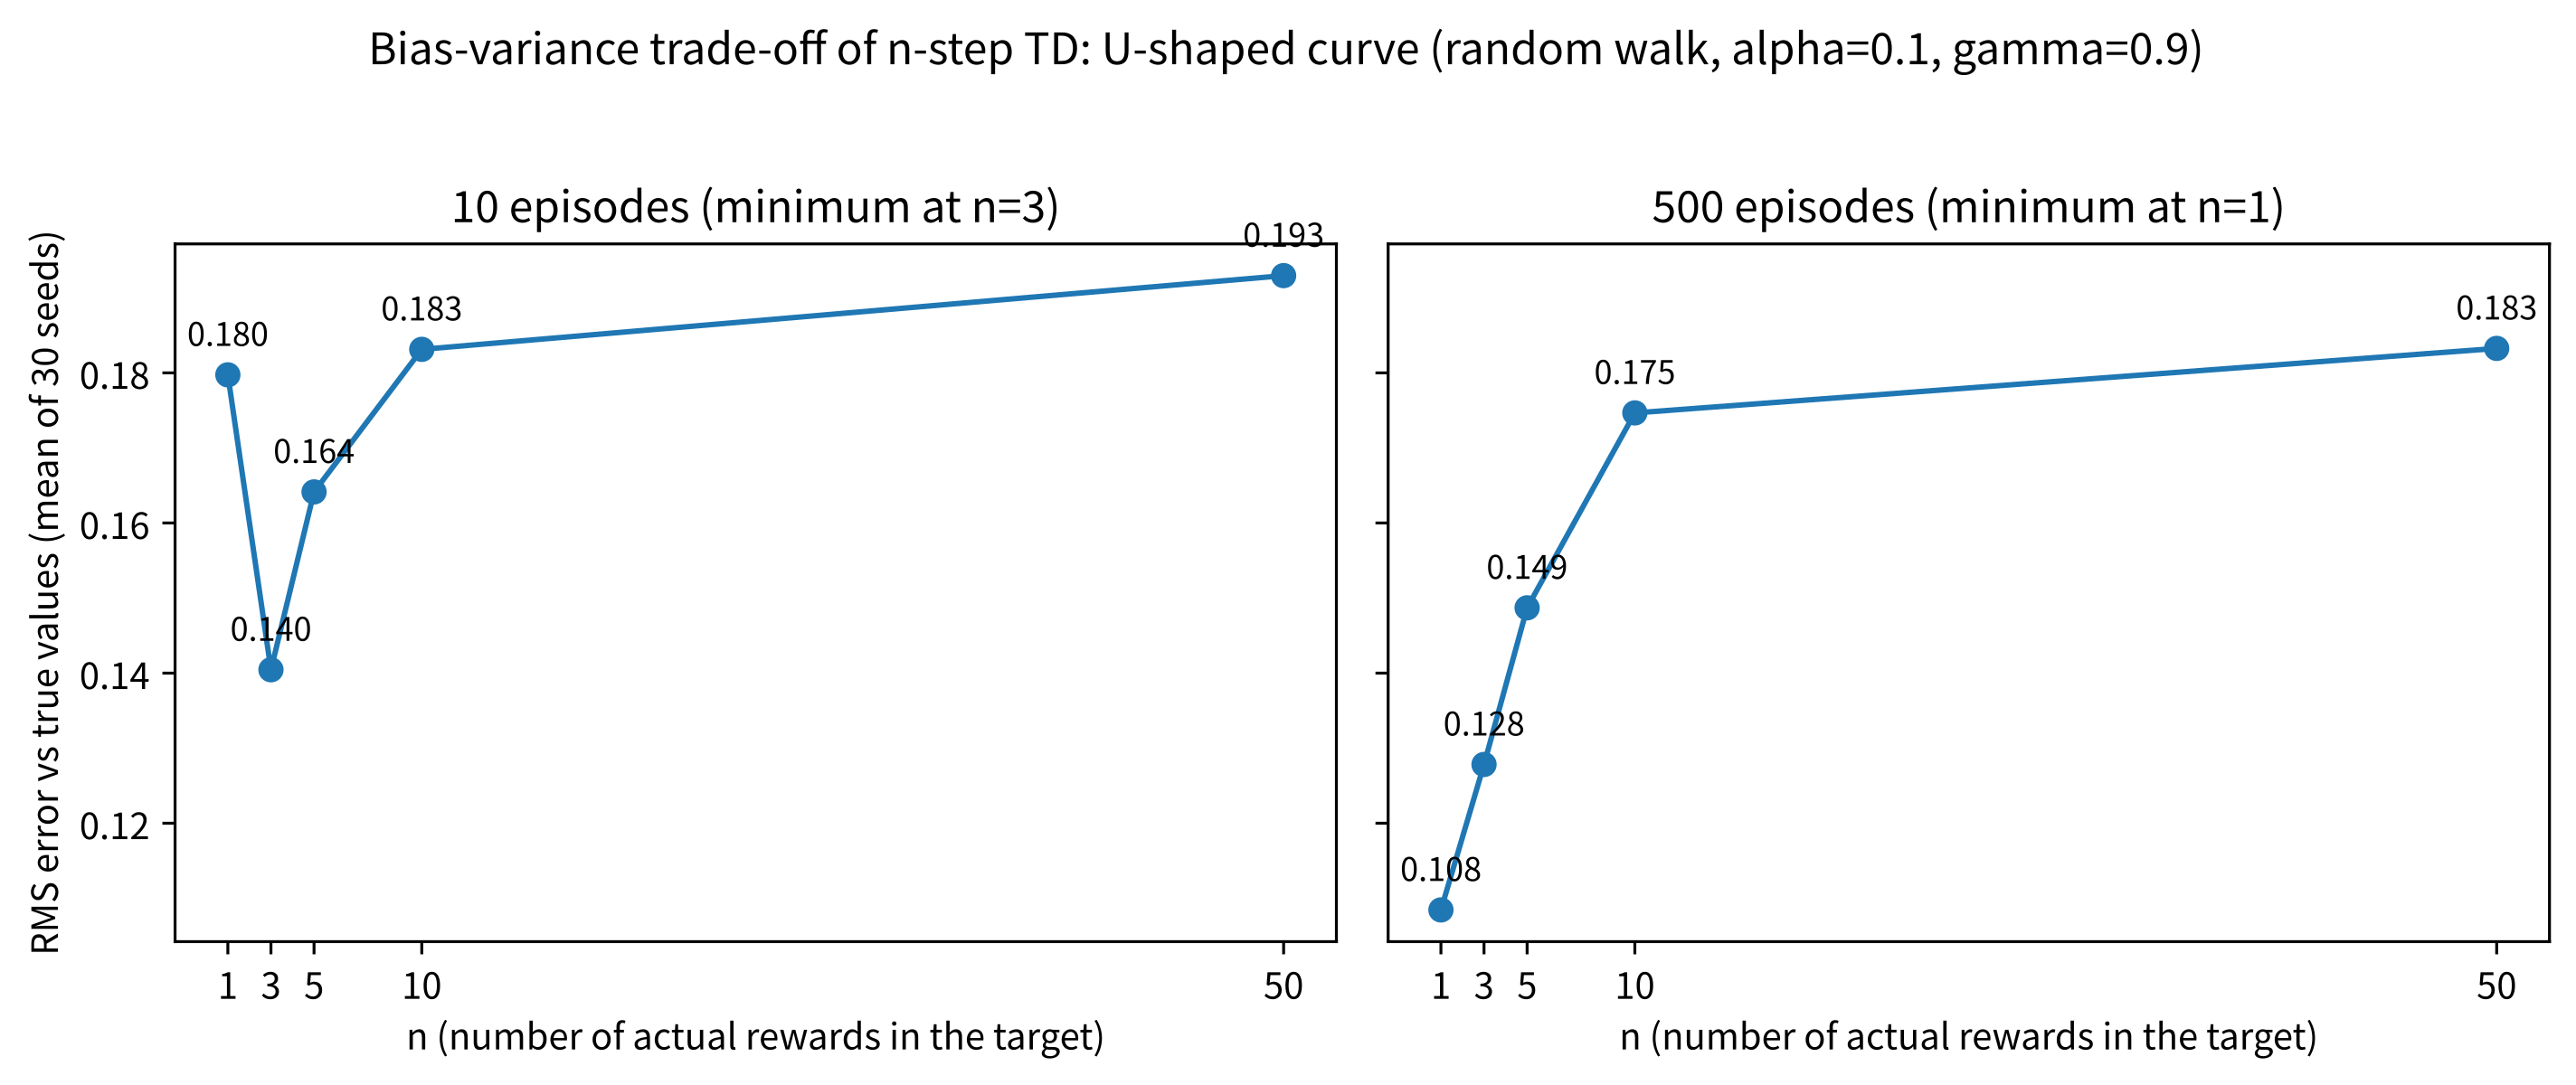
\includegraphics[width=\linewidth]{ch07_1_nstep_ucurve.png}
      {\footnotesize (좌) 10 에피소드: 최저점 $n=3$.
      (우) 500 에피소드: 최저점이 $n=1$ 쪽으로 \textbf{이동}
      ($n=1$: 0.268, $n=3$: 0.336, $n=50$: 0.457).}
    \end{column}
  \end{columns}
  \vskip0.4em
  \begin{itemize}
    \item $n=1$: 추정치 의존(편향)이 10 에피소드로는 씻겨나감
      부족. $n=50$: 분산이 너무 커서 적은 에피소드로 불안정.
    \item 데이터가 쌓이면 ``갱신이 잦고 분산 작은'' TD(0)의 이점이
      살아나 최저점이 $n=1$ 쪽으로 이동. 큰 $n$ 패널티는 예산이
      커져도 크게 줄지 않음.
  \end{itemize}
\end{frame}

\begin{frame}{결론: 보편적인 최적 $n$은 없다}
  \begin{block}{핵심}
    \kq{최적 $n$은 에피소드 예산 · 환경의 확률적 정도 · 할인율에
    따라 움직이는 하이퍼파라미터다.}
    이것이 실전에서 $n$을 검증으로 튜닝해야 하는 이유이며, 7.2의
    적격흔적이 ``$n$을 고르는 문제'' 자체를 피하는(모든 $n$을 흔적으로
    가중합) 대안인 이유이기도 하다.
  \end{block}
  \vskip0.6em
  \kb{$n$을 고르는 경험칙}
  \begin{itemize}
    \item (i) 에피소드 \textbf{짧고} 경험 \textbf{많다}: $n=\infty$(MC)나
      작은 $n$(TD(0))이 안전 --- 편향을 씻어낼 데이터가 있으므로.
    \item (ii) 에피소드 \textbf{길고} 경험 \textbf{적다}: 중간 $n$(3$\sim$10)이
      편향을 줄이면서 분산을 관리.
    \item (iii) 에피소드 \textbf{끝이 없다}(continuing task): MC 자체가
      불가능 $\Rightarrow$ 유한 $n$ 또는 적격흔적(7.2).
  \end{itemize}
  {\footnotesize 실전 DQN(Mnih et al., 2015) 계열에서도 n-step 리턴은
  기본 옵션, 보통 3$\sim$10 범위로 튜닝.}
\end{frame}

\begin{frame}{자주 하는 실수 (1/2)}
  \begin{itemize}
    \item \textbf{할인 지수를 잘못 세기.} \texttt{i - tau - 1}로 쓰면
      $n=1$이어도 \textbf{편향된 목표값}. 2000 에피소드 후에도 참값
      미도달. ``왜 안 수렴하지?'' $\to$ \textbf{먼저 지수를 확인}.
    \item \texttt{tau = t}(지금 상태를 지금 갱신)로 쓰기.
      $G_t^{(n)}$은 $R_t,\dots,R_{t+n-1}$이 다 모인 시점
      ($t+n-1$)에야 계산됨. \texttt{tau = t}면 아직 모이지 않은
      보상을 참조 $\to$ 인덱스 에러, 또는 0으로 채워져 편향.
      \textbf{\texttt{tau = t - n + 1}이 정확}.
  \end{itemize}
\end{frame}

\begin{frame}{자주 하는 실수 (2/2)}
  \begin{itemize}
    \item \textbf{보상 합 상한 확인 안 하기.} 끝 \textbf{근처}에서는
      남은 보상이 $n$개보다 적음(예: $n=3$인데 2스텝 남음).
      \texttt{min(tau + n, len(rewards))}로 안 걸면 인덱스 에러 또는
      ``없는 보상''을 0으로 처리. 추정치 항도 \texttt{tau + n < T}
      없으면 종료 후 $V$ 더하기 / 없는 인덱스 참조.
    \item \textbf{``$n$ > 에피소드 길이면 갱신 안 된다''는 오해.}
      갱신은 모든 이동 상태마다 정확히 1번(꼬리 갱신으로 절단
      목표값 처리). $n$이 바꾸는 것은 횟수가 \textbf{아니라} 시차와
      목표값 구성.
  \end{itemize}
\end{frame}

\begin{frame}{자주 하는 실수 (3/3) + 실습}
  \begin{itemize}
    \item \textbf{``이 환경에서 $n=3$이 최적''을 일반화.} U자 최저점은
      예산·환경에 따라 움직임(10 에피소드 $\to$ $n=3$, 500 에피소드
      $\to$ $n=1$). 실전 표준: \textbf{검증 데이터로 $n$을 튜닝}.
  \end{itemize}
  \vskip0.6em
  \begin{block}{실습: U자 곡선을 직접 만들어보기}
    \begin{enumerate}
      \item 같은 random walk에서 $n \in \{1,3,5,10,50\}$, 10 에피소드
        ($\alpha=0.1$, $\gamma=0.9$, 30 seed 평균) $\to$ RMS 비교.
        최저점 $n=3$, RMS 0.3061 재현.
      \item \textbf{추가 과제}: 에피소드 10 $\to$ 500으로 늘려 다시
        그리면 최저점 $n=1$으로 이동. ``실전에서 $n$을 고를 때 어떤
        상황을 고려해야 하는가''를 한 문장으로 설명.
        (힌트: 예산 적을 때/많을 때 최저점 \textbf{위치}가 어떻게
        달라지는가? 왜?)
    \end{enumerate}
  \end{block}
\end{frame}

\begin{frame}{확인 문제 (1/2)}
  \begin{enumerate}
    \item \kb{$n=1$이 정확히 TD(0)임을 코드로 확인.} \texttt{n=1}로
      실행하고 갱신에 쓰인 $G$가
      $R_\tau + \gamma V(s_{\tau+1})$과 같은지 한 스텝 추적.
      (힌트: \texttt{tau + 1 < T}일 때만 추정치 항 추가. 마지막
      스텝에서는 $G = R_\tau$만 됨 --- ``터미널 $V$는 0''과 일치하는가?)
    \item \kb{$n \to \infty$가 MC임을 확인.} 에피소드가 길이 $T$에서
      끝나면($V(s_T)=0$), $n \ge T$일 때 목표값이 실제 리턴
      $G_t = \sum_{k=0}^{T-t-1} \gamma^k R_{t+k}$과 같은지 보여라.
  \end{enumerate}
\end{frame}

\begin{frame}{확인 문제 (2/2)}
  \begin{enumerate}
    \setcounter{enumi}{2}
    \item \kb{보상 가중치 버그의 효과.} \texttt{gamma ** (i - tau)}를
      \texttt{(i - tau - 1)}로 바꾸고 $n=1$, 2000 에피소드 $\to$ 참값
      미도달 확인. ``목표값의 편향이 \textbf{수렴 고정점 자체를
      바꾼다}는 점을 어떻게 보여주는지'' 한 문장.
    \item \kb{갱신 횟수 세기.} 에피소드 길이 $T$에서
      $n=1$, $n=3$, $n=T+1$ 각각이 \textbf{몇 번} 갱신되는지 코드
      추적. (힌트: $\tau$의 범위와 \texttt{break} 시점. 세 경우가
      \textbf{모두 같은가?} 같은 이유?)
  \end{enumerate}
\end{frame}

\begin{frame}{자주 묻는 질문 (1/2)}
  \begin{itemize}
    \item \kq{n-step TD도 부트스트래핑인가?} --- 그렇다. $n < \infty$
      하면 목표값에 추정치 $V(s_{t+n})$이 들어 있으므로.
      $n\to\infty$(끝까지 실제 보상만)일 때만 순수 MC.
    \item \kq{갱신 횟수는 TD(0)·MC와 어떻게 다른가?} --- \textbf{같다}.
      $T$ 이동 상태면 모두 $T$번. n-step은 첫 $n-1$ 상태가 ``늦어지는''
      뿐이지 사라지지 않음(꼬리 갱신까지). $n$이 바꾸는 것은 시차와
      목표 구성. MC는 갱신 \textbf{시점}이 끝난 뒤라는 점만 다름.
  \end{itemize}
\end{frame}

\begin{frame}{자주 묻는 질문 (2/2)}
  \begin{itemize}
    \item \kq{실전에서는 $n$을 얼마로?} --- 후보 4$\sim$10개를
      \textbf{검증 성능}으로 비교. 이 절의 실습이 그 튜닝의 축소판.
      DQN 구현 중엔 버퍼에서 미니배치를 이어붙여 n-step 목표값을
      만드는 변형도 (Ch.\,9 실습에서 마주침).
    \item \kq{``$n$이 크면 분산 큼''은 갱신당 변동이 크다는 뜻인가?}
      --- 그렇다. $n$ 스텝치 전이·보상 무작위성이 합쳐짐(보상 0의
      스텝도 ``어디로 갔는가''의 전이 무작위성은 누적). 같은 총
      정보를 작은 덩어리(잦은 갱신) vs 큰 덩어리(드문 큰 갱신)로
      나누는 것 = ML1 Ch.\,9의 \textbf{배치 크기 트레이드오프}와
      같은 구조.
    \item \kq{적격흔적(7.2)은 정말 같은 것을 계산하나?} --- ``같은
      효과(모든 $n$ 가중합)를 \textbf{다른 순서}로 만든다''가 정확.
  \end{itemize}
\end{frame}

\section{7.2 적격흔적과 파라미터 튜닝 실습}

\begin{frame}{7.2의 두 가지}
  \begin{itemize}
    \item 첫째, ``$n$을 몇으로 잡을지''는 \textbf{직감으로 고를 수
      없다} --- 데이터로 확인해야 하는 \kb{하이퍼파라미터}. $n$(7.1의
      다이얼)과 $\lambda$(아래 적격흔적의 다이얼)를 바꿔가며,
      \textbf{20회 반복 평균}으로 U자 꼭짓점을 찾는 튜닝 실습.
    \item 둘째, $n$ 하나를 고르는 대신 \textbf{모든 $n$을 동시에}
      처리하는 \kb{적격흔적(eligibility trace)}:
    \item ``이 상태가 \textbf{얼마나 자주}, \textbf{얼마나 최근에}
      방문됐는가''를 기록한 흔적 $e(s)$로, TD 오차가 발생하면 \textbf{
      흔적 크기에 비례해 모든 상태를 동시에} 갱신.
  \end{itemize}
  \vskip0.8em
  \begin{block}{이 절의 주제 하나}
    \kq{편향-분산 트레이드오프(ML1 Ch.\,4.1)를 ``구체적인 숫자''로
    만나는 방법.}
  \end{block}
\end{frame}

\begin{frame}{실습: $n$을 바꿔가며 최적 지점 찾기}
  \begin{itemize}
    \item 같은 7-state random walk 환경. 참고: 이 절의 설정에서는
      \textbf{참값 $V(s) = s/6$}(예: $V(3)=0.5$)이 정확히 알려져
      있음.
    \item \texttt{n\_step\_td}로 10 에피소드 학습, $n$별 RMS 오차,
      \textbf{20회 반복 평균}:
  \end{itemize}
  \vskip0.4em
  \small
  \begin{tabular}{@{}ll@{}}
    \toprule
    $n$ & 평균 RMS 오차 \\
    \midrule
    1 & 0.3410 \\
    3 & 0.1830 \\
    \textbf{5} & \textbf{0.1687} $\leftarrow$ 최적 \\
    10 & 0.1883 \\
    50 & 0.2178 \\
    \bottomrule
  \end{tabular}
  \vskip0.8em
  \begin{itemize}
    \item 다시 \textbf{U자} --- 양 극단($n=1$, $n=50$)보다 중간
      ($n=5$)이 최저. (7.1의 30 seed 실험에선 $n=3$이 최저였음 ---
      설정·시드 수에 따라 바닥 위치가 미세하게 움직임.)
    \item 이 표가 아래 그림의 \textbf{왼쪽 패널}을 그대로 그린 것.
  \end{itemize}
\end{frame}

\begin{frame}{적격흔적: 모든 $n$을 동시에}
  \begin{block}{TD($\lambda$)의 두 갱신식}
    \[
    e(s) \leftarrow \gamma\lambda\, e(s) + \mathbb{1}[s = s_t],
    \qquad
    V(s) \leftarrow V(s) + \alpha\, \delta_t\, e(s)
    \ \ (\text{모든 } s \text{에 대해})
    \]
  \end{block}
  \begin{itemize}
    \item $\lambda \in [0,1]$이 \textbf{새로운 다이얼}:
      $\lambda=0$ $\Rightarrow$ 흔적이 매 스���프 거의 사라져
      \textbf{TD(0)}, $\lambda=1$ $\Rightarrow$ 흔적이 안 줄어
      \textbf{MC에 가까움}.
    \item 이름 TD($\lambda$)가 바로 이 다이얼에서 왔음.
    \item n-step TD = ``$n$ 하나 고정해서 \textbf{전방(forward)}으로
      내다봄'' / 적격흔적 = ``과거 방문 이력에 흔적을 남기고
      \textbf{후방(backward)}으로 갱신을 퍼뜨림'' --- 사실상 같은
      효과(전방/후방 관점의 등가성; 증명은 이 학기 범위 밖).
  \end{itemize}
\end{frame}

\begin{frame}{기원: ADALINE의 ``자격 있는 시냅스''}
  \begin{itemize}
    \item 이름이 생소해 보이지만 기원은 \textbf{1980년대 초} ---
      Barto, Sutton, Anderson (1983$\sim$89) 논문.
    \item ADALINE(최소제곱학습기)에 ``그 시점에 학습에
      \textbf{자격(eligibility)}이 있는 시냅스가 어디인가''를 기록하는
      장치를 처음 도입.
    \item 즉, 강화학습 TD($\lambda$)가 아니라
      \textbf{``어떤 시냅스가 지금 보상을 받을 자격이 있는가''를
      묻던 신경망의 부가장치}였던 셈.
    \item ``어떤 \textbf{상태}가 지금 TD 오차에 기여할 자격이 있는가''
      로 옮겨온 것이 지금의 적격흔적.
  \end{itemize}
  \vskip0.8em
  \kq{``자격을 남기고, 나중에 그 자격만큼 크레딧을 배분한다''.}
\end{frame}

\begin{frame}{손으로 추적: 3 $\to$ 2 $\to$ 3 $\to$ 4}
  \begin{itemize}
    \item 같은 random walk. 한 에피소드에서 상태
      $3 \to 2 \to 3 \to 4$ 순서 방문(중간 상태라 보상 전부 0).
    \item $\gamma=1$, $\lambda=0.5$, $\alpha=0.1$, $V$·$e$는 0에서
      시작. 각 스텝의 TD 오차 $\delta_t$가 이미 계산됐다고 놓고,
      \textbf{$e$가 어떻게 변하고 $V$ 갱신에 어떻게 쓰이는가}만
      추적.
    \item 갱신 순서(매 스텝): \textbf{(1) $\gamma\lambda$로 감쇠
      $\to$ (2) 현재 상태 $+1$ $\to$ (3) 모든 $s$에
      $V(s) \mathrel{+}= \alpha\,\delta_t\,e(s)$}.
  \end{itemize}
  {\footnotesize 다음 3프레임에 표를 $t=0$~2, $t=3$으로 나눠
  보여주고, 각 행의 계산을 확인한다.}
\end{frame}

\begin{frame}{추적 표 (1/2): $t=0$ $\sim$ 2}
  \scriptsize
  \begin{tabular}{@{}clll@{}}
    \toprule
    스텝 $t$ & 현재 상태 & $\delta_t$ & 이번 스텝 $V$ 갱신 \\
    \midrule
    0 & 3 & $+0.4$ & $e(3)=1$:  $V(3)\mathrel{+}=0.1\cdot0.4\cdot1=+0.040$ \\
    1 & 2 & $+0.3$ & $e(2)=1, e(3)=0.5$:  $V(2)\mathrel{+}=+0.030$,  $V(3)\mathrel{+}=0.1\cdot0.3\cdot0.5=+0.015$ \\
    2 & 3 & $+0.5$ & $e(2)=0.5, e(3)=1.25$:  $V(2)\mathrel{+}=+0.025$,  $V(3)\mathrel{+}=0.1\cdot0.5\cdot1.25=+0.0625$ \\
    \bottomrule
  \end{tabular}
  \vskip0.8em
  \begin{itemize}
    \item $t=1$: $t=0$의 $e(3)=1$이 $0.5$로 \textbf{감쇠}, 현재 2에
      $+1$.
    \item $t=2$: $e(3)=0.5\cdot0.5=0.25$로 감쇠한 뒤 \textbf{재방문}에
      $+1$ $\Rightarrow$ $e(3)=\mathbf{1.25}$ --- \textbf{방문 빈도가
      흔적에 누적}.
  \end{itemize}
\end{frame}

\begin{frame}{추적 표 (2/2): $t=3$에서 한 오차, 세 상태}
  \scriptsize
  \begin{tabular}{@{}cll@{}}
    \toprule
    스텝 $t$ & 현재 상태 & $\delta_t$ & 이번 스텝 $V$ 갱신 \\
    \midrule
    3 & 4 & $+0.2$ & $e(2)=0.25, e(3)=0.625, e(4)=1$:  
      $V(2)\mathrel{+}=+0.005$,  $V(3)\mathrel{+}=+0.0125$,  
      $V(4)\mathrel{+}=0.1\cdot0.2\cdot1=+0.020$ \\
    \bottomrule
  \end{tabular}
  \vskip0.8em
  \begin{itemize}
    \item \textbf{하나의} TD 오차 $\delta_3=0.2$가 \textbf{세 개} 상태
      (2, 3, 4)를 동시에 갱신:
      \begin{itemize}
        \item 현재 상태 4(흔적 1)가 가장 크게,
        \item 직전 상태 3(0.625)이 그다음,
        \item 한 번 더 지난 상태 2(0.25)가 가장 작게.
      \end{itemize}
      이것이 ``\textbf{후방으로 크레딧을 퍼뜨린다}''는 뜻.
    \item $\lambda=0.5$라 기억이 1$\sim$2 스텝 전까지만 유효 ---
      $\lambda=0.9$로 올리면 훨씬 길어짐.
  \end{itemize}
\end{frame}

\begin{frame}{$\lambda$가 $n$을 어떻게 ``대체''하는가}
  \begin{itemize}
    \item n-step TD의 목표값 $G_t^{(n)}$: \textbf{단 하나의} n-step
      리턴(정확히 $n$ 스텝만 보고 나머지는 추정치).
    \item 적격흔적: 흔적 감쇠율 $\gamma\lambda$ 덕분에 $t$ 스텝 전에
      방문한 상태의 흔적은 대략 $(\gamma\lambda)^t$로 감소.
  \end{itemize}
  \vskip0.6em
  \begin{block}{TD($\lambda$)의 목표 = 한 줄}
    \[
    \text{TD}(\lambda)\text{의 목표} \;\approx\;
    \text{``모든 $n$-step 목표의 가중평균, }
    n\text{에 대한 가중치} \propto \lambda^{\,n-1}\text{''}
    \]
  \end{block}
  \begin{itemize}
    \item $\lambda$ \textbf{작으면} 가중치가 빠르게 $\lambda^{n-1}$로
      죽어 실질적으로 짧은 $n$(TD(0) 쪽)만 사용.
    \item $\lambda$ \textbf{크면} 긴 $n$에도 충분한 가중치 $\Rightarrow$
      MC 쪽으로 이동.
  \end{itemize}
\end{frame}

\begin{frame}{``하나를 고르는 문제''에서 ``분포의 형태''로}
  \begin{itemize}
    \item $n$-step이 \textbf{``하나의 $n$을 고르는''} 문제였다면,
      TD($\lambda$)는 \textbf{``가중치 분포 $\lambda^{n-1}$의 형태''}를
      $\lambda$ 하나로 조절하는 문제.
    \item 같은 편향-분산 트레이드오프를, \textbf{하나를 고르는 문제에서
      분포의 형태를 고르는 문제로 승화}시킨 것.
  \end{itemize}
  \vskip0.8em
  \begin{block}{직접 확인해야 할 한 줄}
    $\lambda$를 $n$으로 환산하는 근사 대응: TD($\lambda$)의
    \textbf{유효 수명(effective horizon) $\sim 1/(1-\lambda)$ 스텝}.
    $\lambda=0.8$이면 대략 $1/(1-0.8) = 5$ 스텝 전후 --- 이번 실험에서
    $n=5$가 최적, $\lambda=0.8$이 최적인 것과 \textbf{동일한 방향}.
    정확한 1:1 변환은 아니지만, ``$\lambda=0.8$이 5스텝 정도
    내다보는 것과 비슷하다''는 직관은 잡아둠.
  \end{block}
\end{frame}

\begin{frame}{실습: $\lambda$를 바꿔가며 최적 지점 찾기}
  \begin{itemize}
    \item $\lambda$도 하이퍼파라미터 $\Rightarrow$ $n$과 똑같이
      \textbf{데이터로 고름}.
    \item 같은 random walk, 10 에피소드, $\alpha=0.2$, $\gamma=1$,
      $\lambda$ 0$\sim$1, \textbf{20회 반복 평균} RMS:
  \end{itemize}
  \vskip0.4em
  \small
  \begin{tabular}{@{}ll@{}}
    \toprule
    $\lambda$ & 평균 RMS 오차 \\
    \midrule
    0.0 (TD(0)와 동일) & 0.3172 \\
    0.2 & 0.2790 \\
    0.4 & 0.2329 \\
    0.6 & 0.1774 \\
    \textbf{0.8} & \textbf{0.1377} $\leftarrow$ 최적 \\
    1.0 (사실상 MC) & 0.2674 \\
    \bottomrule
  \end{tabular}
  \vskip0.8em
  \begin{itemize}
    \item 다시 \textbf{U자}. 좌측 $\lambda=0$은 정확히 TD(0)($n=1$,
      $\alpha=0.2$ 결과와 같은 0.3172)라 편향 씻어내지 못함.
      우측 $\lambda=1$은 MC에 가까워 분산 큼.
    \item \textbf{``$\lambda=0.8$이 만능 정답''이 아니다} ---
      환경·에피소드 수(예: 1000)가 바뀌면 U자 바닥은 \textbf{완전히
      다른 위치}로 이동. 에피소드가 충분히 많으면 편향이 씻겨
      $\lambda$를 1에 가깝게(MC 쪽) 가져가도 좋은 경우 많음.
    \item \kq{``데이터로 고르는 것'' 자체가 방법 --- 검증 데이터·
      반복 실험으로 매번 재확인하는 습관이 실전의 본체.}
  \end{itemize}
\end{frame}

\begin{frame}{두 개의 U자 나란히}
  \begin{columns}[T]
    \begin{column}{0.58\textwidth}
      \centering
      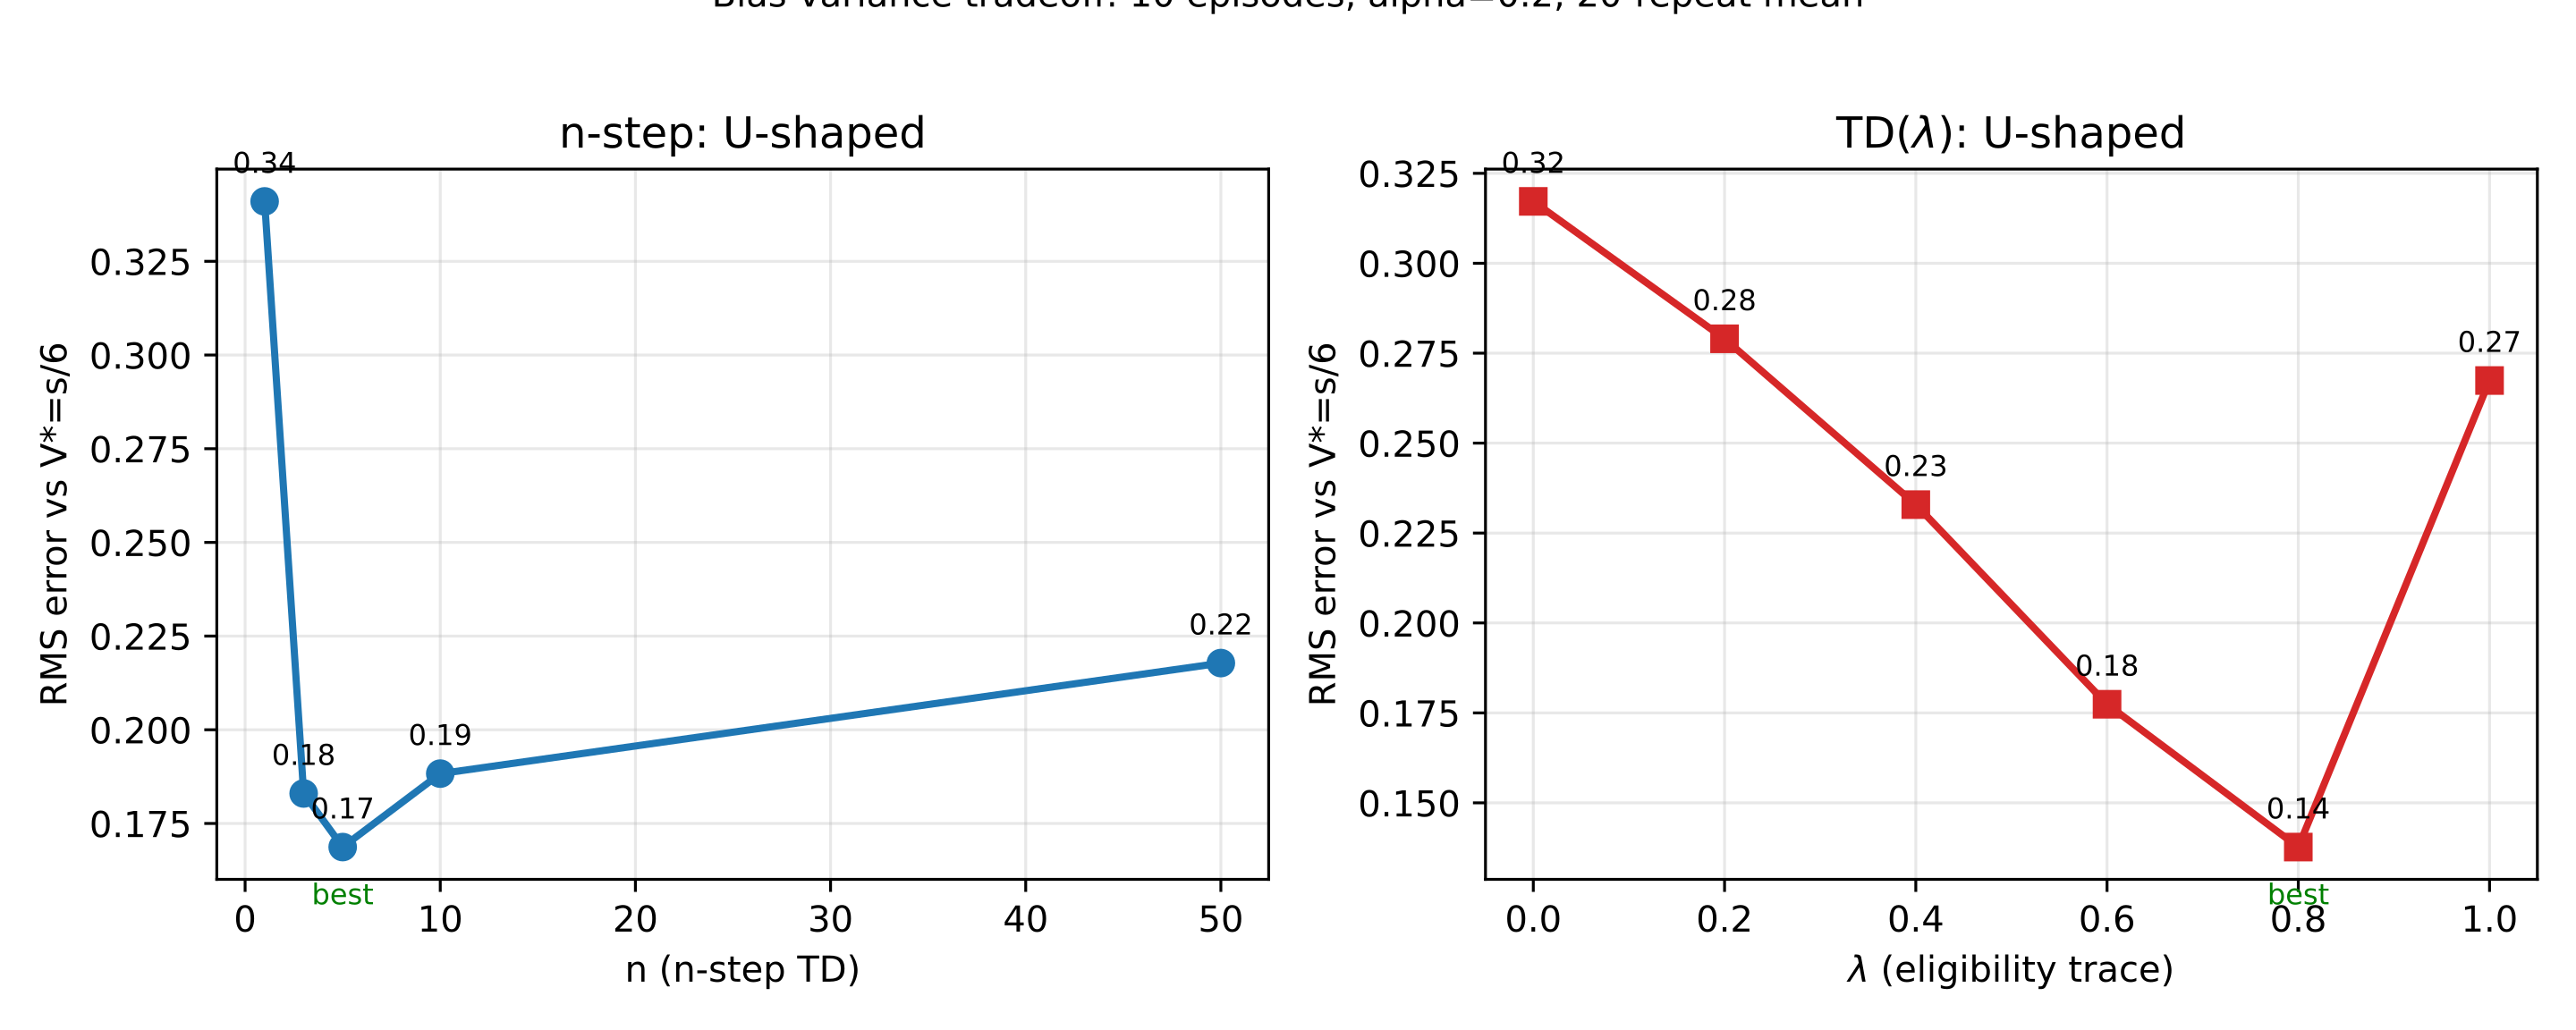
\includegraphics[width=\linewidth]{ch07_2_ucurve.png}
      {\footnotesize (좌) $n$-step: 최저 $n=5$, 0.17.
      (우) TD($\lambda$): 최저 $\lambda=0.8$, 0.14.
      10 에피소드 · $\alpha=0.2$ · 20회 반복 평균.}
    \end{column}
    \begin{column}{0.40\textwidth}
      \begin{block}{두 패널이 나란하니 메시지가 선명하다}
        \kq{$n$을 고르는 일과 $\lambda$를 고르는 일은
        \textbf{같은 편향-분산 트레이드오프의 두 모습}.}
        둘 다 U자. ``$n=5$''와 ``$\lambda=0.8$''은 서로 다른
        문제를 푸는 게 아니라, \textbf{``같은 U자에서 지금 이
        데이터양·이 문제에서 바닥이 어디인지''를 각각의 다이얼
        위에서 재확인한 결과}일 뿐.
      \end{block}
    \end{column}
  \end{columns}
\end{frame}

\begin{frame}{단 한 번의 실행은 믿지 마라}
  \begin{itemize}
    \item 위 실습 코드($\alpha=0.2$, 10 에피소드)를 \textbf{단 한 번}
      (시드 0)만 돌려 마지막 $V$를 참값 $V(s)=s/6$과 비교:
  \end{itemize}
  \vskip0.3em
  \small
  \begin{tabular}{@{}ll@{}}
    \toprule
     & $V(1\sim5)$ (RMS) \\
    \midrule
    $n=1$ & 0.00  0.02  0.08  0.16  0.48  (0.370) \\
    $n=5$ & 0.05  0.07  0.30  0.44  0.67  (0.201) \\
    $n=50$ & 0.12  0.20  0.37  0.56  0.81  \textbf{(0.099) $\leftarrow$ 이번엔 이게 제일 좋다} \\
    참값 & 0.17  0.33  0.50  0.67  0.83 \\
    \bottomrule
  \end{tabular}
  \vskip0.8em
  \begin{itemize}
    \item 단일 실행에선 \textbf{$n=50$이 제일 정확} --- 이 실행만
      보고 튜닝했다면 $n=50$을 골랐을 것.
    \item 그러나 20회 평균에선 $n=50$은 0.2178로 \textbf{양 끝 중
      나쁜 쪽}. ``이번엔 운이 좋아 $n=50$이 잘 된'' \textbf{단일 시드가
      전체 U자를 완전히 역전}시킨 것.
  \end{itemize}
  {\footnotesize 아래 그림은 이 단일 실행(시드 0)의 세 곡선을 참값과
  함께 그린 것 --- $n=50$(빨강)이 이번 실행에선 참값에 가장 가까움.}
\end{frame}

\begin{frame}{단일 시드 vs 20회 평균}
  \begin{columns}[T]
    \begin{column}{0.56\textwidth}
      \centering
      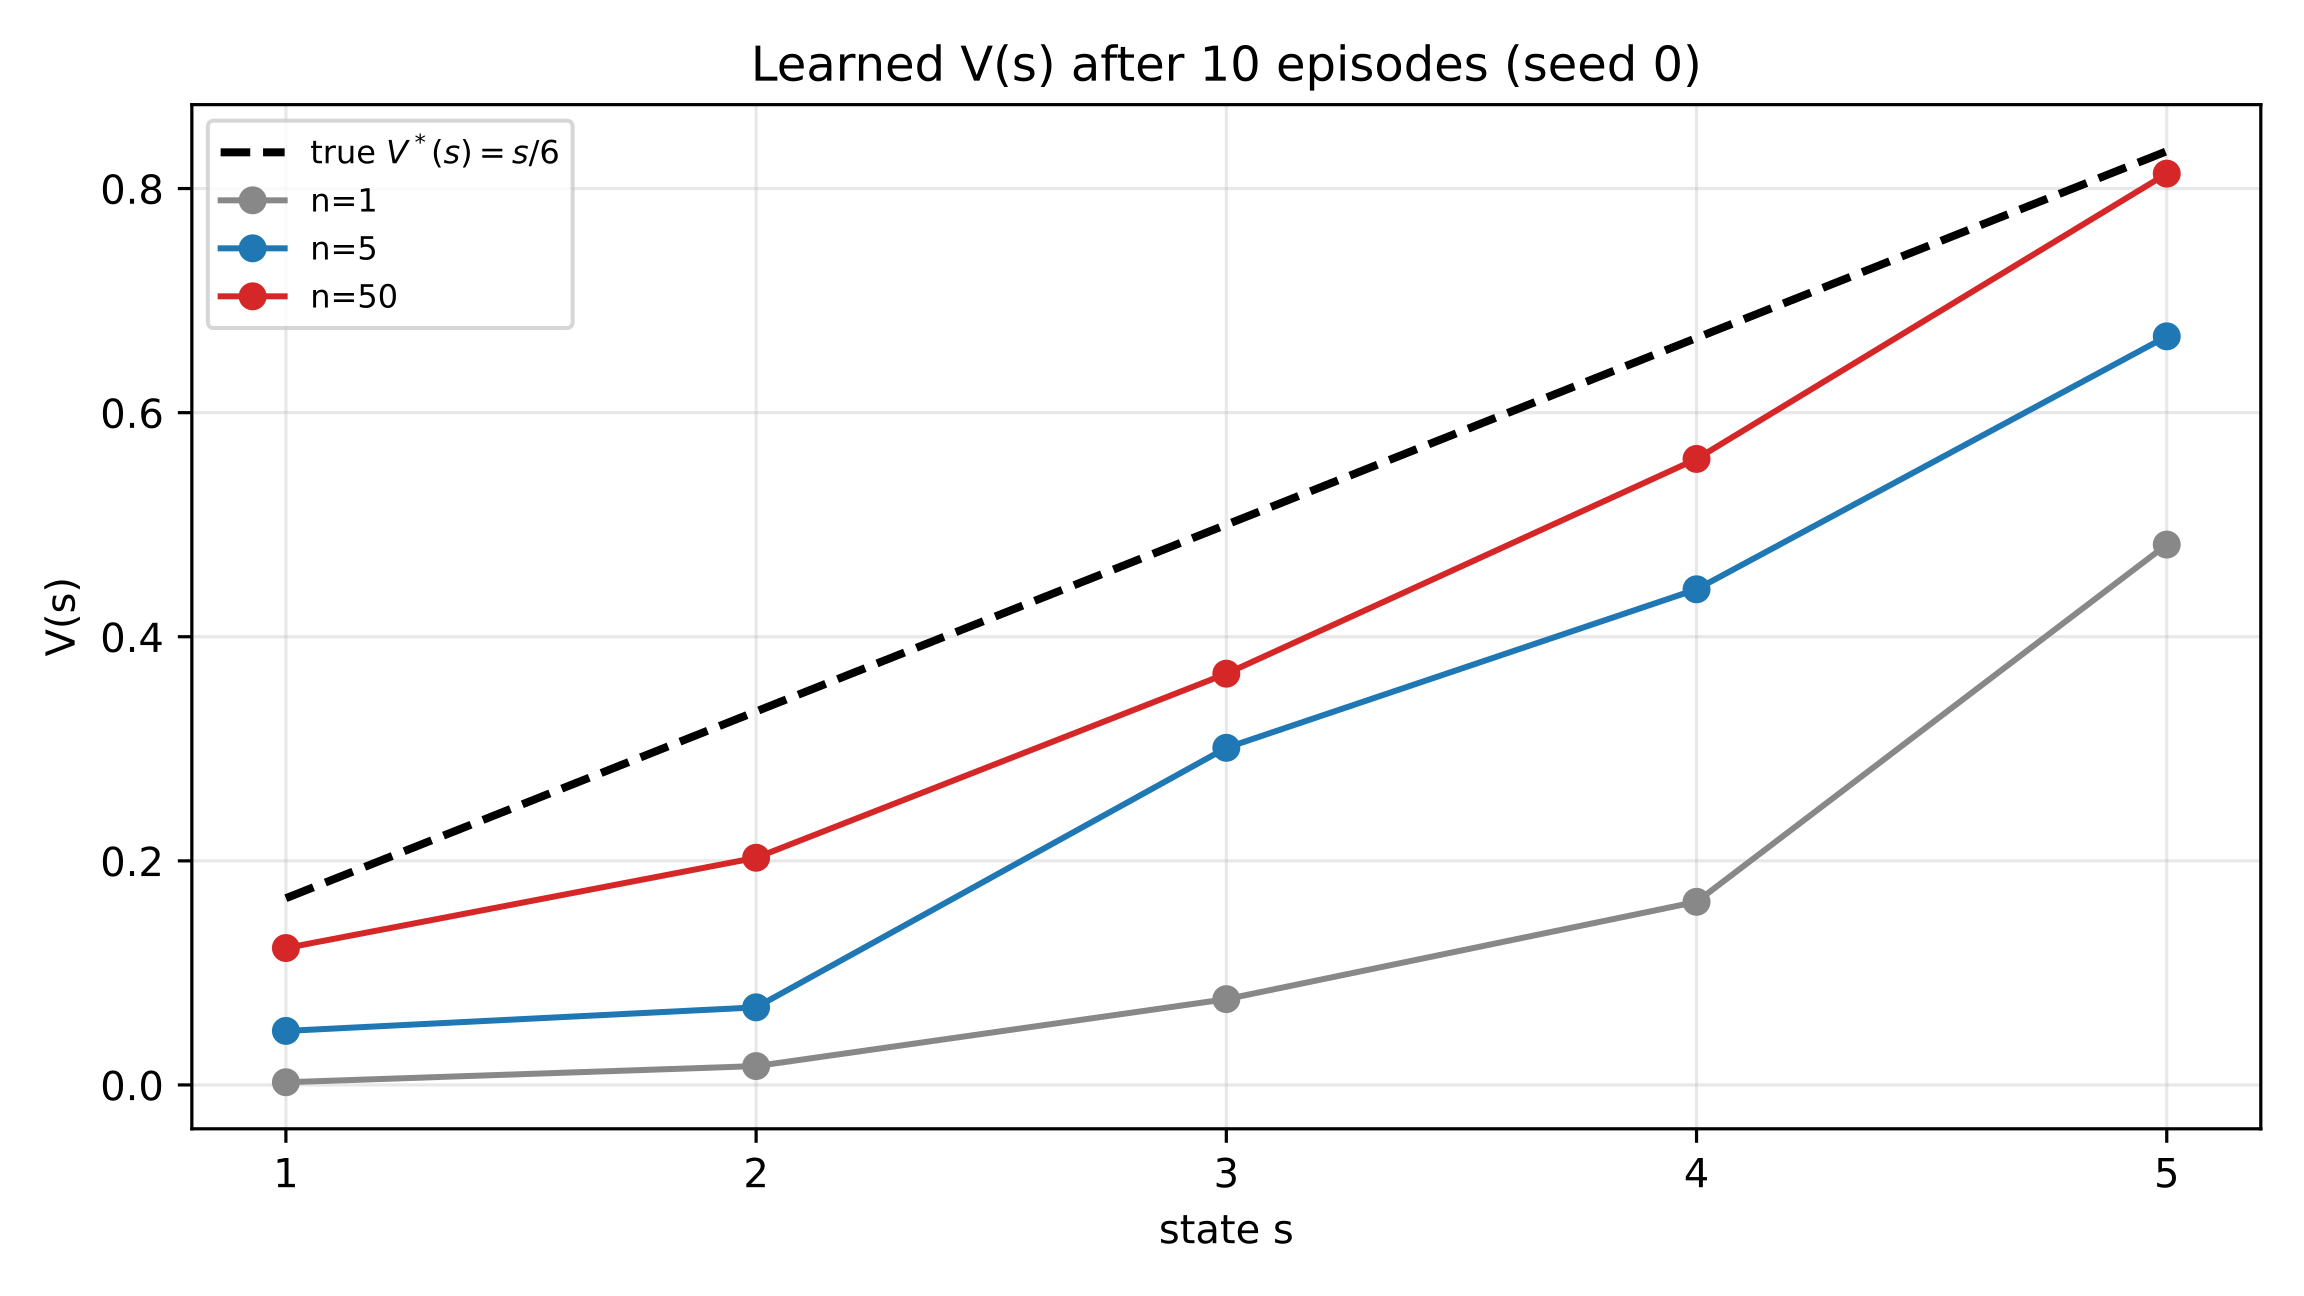
\includegraphics[width=\linewidth]{ch07_2_vconverge.png}
      {\footnotesize 단일 실행(시드 0, $\alpha=0.2$, 10 에피소드)의
      학습 $V(s)$와 참값 $V^*=s/6$. $n=1$(회색)은 거의 0에서
      움직이지 못해 큰 편향, $n=5$(파랑)은 중간, $n=50$(빨강)은
      이번 실행에선 참값에 가장 가까움.}
    \end{column}
    \begin{column}{0.42\textwidth}
      \begin{block}{함정의 본질}
        \kq{하이퍼파라미터를 고르면서 단일 실행(단일 시드, 단일
        검증집합)에 의존하면, ``U자를 찾겠다''는 전제가
        \textbf{완전히 무너진다}.}
        \vskip0.4em
        \textbf{최적 지점을 찾는 실험은 반드시 여러 시드/반복으로
        평균내야 한다} --- 이 절이 실제로 강조하는 튜닝의
        전제 조건.
      \end{block}
    \end{column}
  \end{columns}
\end{frame}

\begin{frame}{이 절의 하이퍼파라미터 지도}
  \small
  \begin{tabular}{@{}llll@{}}
    \toprule
    방법 & 목표값 & 하이퍼파라미터(다이얼) & 이 절의 결과 \\
    \midrule
    TD(0) & $r+\gamma V(s')$ & ---($n=1$) & U의 좌측 극단 \\
    n-step TD & $n$ 스텝 실제 + 나머지 추정 & $\mathbf{n}$ & U의 바닥 $n\approx 5$ \\
    TD($\lambda$) & 모든 $n$의 가중평균 & $\boldsymbol{\lambda}$ & U의 바닥 $\lambda\approx 0.8$ \\
    (참고) MC & 실제 리턴 $G_t$ & ---($n=\infty$, $\lambda=1$) & U의 우측 극단 \\
    \bottomrule
  \end{tabular}
  \vskip1em
  \begin{itemize}
    \item 여기에 \kb{$\alpha$(학습률)}과 \kb{에피소드 수}가 겹침.
    \item $\alpha$는 U자의 \textbf{깊이}를, 에피소드 수는 U자의
      \textbf{바닥 위치}를 동시에 바꿈 --- 에피소드가 늘면 편향이
      씻겨 나와 바닥이 \textbf{우측(긴 부트스트래핑)}으로 이동.
    \item ``$n=5$, $\lambda=0.8$''은 \textbf{이 실험(10 에피소드,
      $\alpha=0.2$)에서의 답}이지 보편 정수가 아님.
  \end{itemize}
  {\footnotesize 실정: ``데이터양을 늘릴수록 다이얼을 어떻게
  이동시킬지''를 예상하고 검증 데이터로 확인하는 것이 정석.
  (TD($\lambda$) 심화: Stanford CS234)}
\end{frame}

\begin{frame}{자주 하는 실수 (1/2)}
  \begin{itemize}
    \item \textbf{첫째, ``$\lambda=1$이 편향이 없으니까 무조건
      낫다''.} 편향이 없는 것(MC)은 \textbf{분산이 최대}인 극단.
      10 에피소드라는 \textbf{적은 데이터}에선 분산이 편향보다 더
      먼저 손해를 냄 $\Rightarrow$ U자 우측으로 갈수록 \textbf{오히려
      나빠짐}.
      ``편향만 보고 고르는'' 것은 반쪽짜리 판단. \textbf{항상
      편향과 분산을 합친 총 오차(RMS)로} 봐야 함 --- 이 절의 모든
      표가 RMS로 집계된 이유.
  \end{itemize}
\end{frame}

\begin{frame}{자주 하는 실수 (2/2)}
  \begin{itemize}
    \item \textbf{둘째, 단일 실행(단일 시드)으로 최적 지점 정하기.}
      위 ``단 한 번의 실행은 믿지 마라''가 그대로 실수. 하이퍼파라미터
      실험은 필연적으로 \textbf{여러 시드·반복으로 평균}내야 U자 바닥이
      안정적으로 보임. 하나의 실행은 \textbf{운}.
    \item \textbf{셋째, 흔적 갱신 순서를 뒤집기.} 순서는
      \textbf{``$\gamma\lambda$로 감쇠 $\to$ 현재 상태 $+1$ $\to$
      모든 $s$에 $V \mathrel{+}= \alpha\delta e$''}.
      ``$+1$''을 갱신 \textbf{이후}에 하면, 그 스텝 TD 오차가 현재
      상태 자신에 적용될 때 흔적이 1이 아닌 \textbf{감쇠된 값}이 되어
      $\lambda=0$이 TD(0)와 정확히 같아지지 않음.
      \textbf{건성 체크(sanity check)}:
      \texttt{lambda=0}이 \texttt{n=1}과 RMS가 \textbf{완전히 일치}
      하는지($\alpha=0.2$ 단일 실행에서 0.3696 = 0.3696).
      순서가 바르면 이 일치성이 깨짐.
  \end{itemize}
\end{frame}

\begin{frame}{확인 문제}
  \begin{enumerate}
    \item \kb{왜 U자인가.} 좌측 극단(짧은 부트스트래핑) = \textbf{
      편향}의 문제, 우측 극단(긴 부트스트래핑) = \textbf{분산}의
      문제. 그리고 ``에피소드 1000으로 늘리면 U자 바닥이 어느
      쪽으로 이동할지, 왜'' 한 문장씩.
    \item \kb{흔적의 두 역할.} $t=3$ 행에서 상태 4/3/2의 갱신 크기가
      각각 다른 이유를 \textbf{흔적 값(1, 0.625, 0.25)}을 들어 설명.
      상태 3이 상태 2보다 \textbf{더 큰 누적 갱신}을 받은
      \textbf{두 번째 이유}(감쇠와 \textbf{무관}한 이유) 짚기.
      (힌트: 재방문 $\Rightarrow$ $e(3)=1.25$.)
    \item \kb{코딩.} \texttt{td\_lambda}($\lambda=0$)의 마지막 $V$가
      같은 설정 \texttt{n\_step\_td(n=1)}과 RMS가 일치하는지
      ($<10^{-9}$ 차이) \texttt{assert}로 확인. 이 검증이
      ``적격흔적 코드가 올바른가''를 어떻게 보장하는지 한 문장.
  \end{enumerate}
\end{frame}

\begin{frame}{자주 묻는 질문 (1/2)}
  \begin{itemize}
    \item \kq{에피소드 수가 많으면 $\lambda=1$(MC) 쪽이 좋아지나요?}
      --- MC의 단점은 \textbf{분산}이지 편향이 아님. 에피소드 10개면
      각 갱신이 ``그 에피소드의 운''에 크게 흔들리지만 1000개면
      무작위성이 \textbf{평균에 의해 서로 상쇄}되어 MC의 분산이 거의
      사라짐 $\Rightarrow$ 남는 건 편향뿐(MC는 0) $\Rightarrow$
      $\lambda=1$이 가장 정확. 반대로 에피소드가 적으면 편향·분산
      중 \textbf{어느 쪽이 더 큰 손해인가}가 U자 좌/우 기울기를
      정함.
  \end{itemize}
\end{frame}

\begin{frame}{자주 묻는 질문 (2/2)}
  \begin{itemize}
    \item \kq{``모든 상태 동시 갱신''의 계산 비용은 터지나?}
      --- 갱신 대상 = \textbf{방문한 상태 수}(보통 5개). 매 스텝
      5번 곱셈+덧셈 = TD(0)의 ``매 스텝 1번'' 대비 \textbf{상당히
      가벼운 증가}. 상태 10만 개(고차원 격자) 수준에선 ``모든
      상태 순회''가 병목 $\Rightarrow$ 실전에서는 \textbf{흔적 0인
      상태를 건너뛰는 희소(sparse) 구현}, 또는 DQN처럼
      \textbf{신경망 + 적격흔적 조합}.
      핵심 구조적 아이디어(후방 크레딧 배분)는 그대로,
      계산 표현만 상황에 맞게 최적화.
  \end{itemize}
  \vskip0.8em
  \begin{block}{이 절의 핵심 한 줄}
    \kq{적격흔적은 ``$n$ 하나를 고르는 것''을 ``모든 $n$의 가중분포를
    $\lambda$ 하나로 조절하는 것''으로 승화시킨 기법.}
    분포의 형태($\lambda$) + 학습률($\alpha$) + 데이터량(에피소드 수)
    셋이 \textbf{함께} U자 바닥을 정하므로, 이 셋을 \textbf{데이터로
    튜닝}하는 것이 실전의 전부.
  \end{block}
\end{frame}

\section{7.3 계획과 학습: Dyna-Q}

\begin{frame}{경험을 버리지 않는 법}
  \begin{itemize}
    \item 지금까지의 모델-프리 방법(MC, TD, Q-learning)은 경험을
      \textbf{한 번 쓰고 버림}.
    \item 그런데 한 스텝 $(s,a)\to(r,s')$에는 두 가지가 담겨 있다:
      \begin{itemize}
        \item (1) \textbf{Q를 갱신할 신호}(TD(0) 갱신)
        \item (2) \textbf{환경에 대한 지식} --- ``$(s,a)$를 하면
          대략 $(r,s')$이 나온다''.
      \end{itemize}
      모델-프리는 (2)를 \textbf{버림}.
    \item (2)는 어디에 쓰이는가? --- \textbf{아직 실제로 가보지 못한
      상태의 가치를 추정}하는 데.
  \end{itemize}
  \vskip0.8em
  \begin{block}{\kb{Dyna-Q}(Sutton, 1990 박사논문)}
    이 정보를 간단한 \textbf{모델}로 저장해뒀다가, 실제
    상호작용 사이사이에 \textbf{가상의 추가 학습(계획, planning)}을
    끼워 넣는다.
  \end{block}
\end{frame}

\begin{frame}{왜 모델을 저장하는가 --- 상호작용이 비쌀 때}
  \begin{itemize}
    \item 실제 환경 상호작용의 \textbf{비용이 비쌀수록}, ``간접적으로
      값을 아는 것''의 가치가 큼.
    \item 로봇 한 칸 이동에 몇 초, 실험실 화학 반응은 하루를 넘길
      수 있음.
    \item 실제 스텝 1회당 $Q$ 갱신 횟수를 10배로 늘려주는 것은
      \textbf{학습에 소요되는 실세계 시간을 10분의 1로 줄여주는}
      것과 같음.
  \end{itemize}
  \vskip0.8em
  \begin{block}{Dyna-Q의 계산}
    learning rate를 높이는 대신, \textbf{같은 실제 경험}으로 더 많은
    갱신을 만들어내는 것. 아주 단순한 구조로 해냄:
    \textbf{``본 $(s,a)$의 마지막 $(r,s')$를 기억하는 표''}.
  \end{block}
\end{frame}

\begin{frame}[fragile]{Dyna-Q 코드: 경험 $\to$ 학습 $\to$ 모델 저장 $\to$ 계획}
  \begin{lstlisting}[basicstyle=\ttfamily\scriptsize]
def dyna_q(env_step, n_states, n_actions, n_episodes,
           planning_steps, alpha, gamma, epsilon, start_state):
    Q = [[0.0] * n_actions for _ in range(n_states)]
    model = {}  # (s, a) -> (r, s')  관찰한 것을 그대로 저장
    for _ in range(n_episodes):
        s = start_state
        for _ in range(100):
            a = random.randrange(n_actions) if random.random() < epsilon \
                else max(range(n_actions), key=lambda x: Q[s][x])
            ns, r, done = env_step(s, a)
            Q[s][a] += alpha * (r + gamma * max(Q[ns]) - Q[s][a])  # 1) 실제 학습
            model[(s, a)] = (r, ns)                                 # 2) 모델 갱신
            for _ in range(planning_steps):                         # 3) 계획
                (ps, pa), (pr, pns) = random.choice(list(model.items()))
                Q[ps][pa] += alpha * (pr + gamma * max(Q[pns]) - Q[ps][pa])
            s = ns
            if done:
                break
    return Q
  \end{lstlisting}
  {\footnotesize 결정론적 환경 가정(같은 $(s,a)$은 항상 같은
  $(r,s')$을 냄). \texttt{planning\_steps}가 클수록 실제 스텝 1회당
  경험을 모델을 통해 ``몇 번이고 복습''.}
\end{frame}

\begin{frame}{실제 숫자: 같은 환경, 계획이 있는가}
  \begin{itemize}
    \item 같은 격자 환경에서, \textbf{목표 상태(state 3, 오른쪽으로
      가는 행동)의 $Q$값이 0.5를 넘어서기까지}의 에피소드 수:
  \end{itemize}
  \vskip0.4em
  \small
  \begin{tabular}{@{}ll@{}}
    \toprule
    설정 & 0.5 초과까지 에피소드 \\
    \midrule
    \texttt{planning\_steps=0} (순수 Q-learning) & 253 \\
    \texttt{planning\_steps=10} & \textbf{9} $\leftarrow$ 매 실제
    스텝마다 모델로 10번 추가 학습 \\
    \bottomrule
  \end{tabular}
  \vskip1em
  \begin{block}{핵심}
    \kq{같은 \textbf{실제 경험}으로, 계획이 있는 쪽이 \textbf{훨씬
    더 많은 것}을 뽑아낸다.}
  \end{block}
\end{frame}

\begin{frame}{역사적 맥락: 학습과 계획을 하나의 루프로}
  \begin{itemize}
    \item ``Dyna''라는 이름은 \textbf{1990년 Richard Sutton의
      박사논문}에 등장.
    \item 당시는 \textbf{학습(샘플로)과 계획(모델로)을 서로 다른
      연구 분야}로 봄.
    \item Sutton은 이 둘을 \textbf{하나의 루프} 안에 넣고:
      \begin{block}{Dyna의 구조}
        \textbf{학습이 만든 모델이 계획을 하고, 계획이 학습을
        가속한다.}
      \end{block}
    \item 이후 \textbf{모델 기반 강화학습(model-based RL)의 거의
      모든 변형}은 이 Dyna의 골격(실제 경험 $\leftrightarrow$
      모델로 계획, 두 루프 병행) 위에서 변주.
    \item Ch.\,15.2의 \textbf{AlphaGo/AlphaZero}(Silver et al.,
      2016/2018)의 ``신경망 $\leftrightarrow$ MCTS 탐색이 서로를
      개선''도, 동전이 하나 뒤집힌(신경망 = 모델, MCTS = 계획)
      \textbf{같은 구조}.
  \end{itemize}
\end{frame}

\begin{frame}{손으로 계획 한 스텝: 3상태 예제}
  \begin{itemize}
    \item 상태 $S$(출발) $\to$ $X$ $\to$ $T$(목표, 종료),
      각 상태마다 행동 하나, 전이는 \textbf{결정론적}.
    \[
    S \xrightarrow{a} X \ (\text{보상 } 0), \qquad
    X \xrightarrow{a} T \ (\text{보상 } +1), \qquad
    \gamma = 0.9, \ \alpha = 0.5
    \]
    \item 참값(벨만방정식 \textbf{거꾸로} 쓰기):
      $Q(T)=0$, $Q(X) = 1 + \gamma\cdot 0 = 1$,
      $Q(S) = 0 + \gamma\cdot 1 = 0.9$.
    \item 이 ``\textbf{거꾸로}'' 방향이 핵심 --- 아래에서 실제로
      어떻게 일어나는지 추적.
  \end{itemize}
\end{frame}

\begin{frame}{추적 (1/3): 실제 경험만 있으면 $Q(S)$는 안 움직임}
  \begin{itemize}
    \item 초기 $Q(S)=Q(X)=Q(T)=0$.
    \item 에이전트가 \textbf{실제로} $S\to X$(보상 0) 한 번 경험:
    \[
    Q(S) \leftarrow 0 + 0.5\,(0 + 0.9\cdot Q(X) - 0) = 0
    \]
      $Q(X)$가 아직 0이라 $Q(S)$는 \textbf{안 움직임}.
      \textbf{여기까지가 순수 Q-learning이 할 수 있는 전부}.
  \end{itemize}
  \vskip0.8em
  \begin{itemize}
    \item 이어서 \textbf{실제로} $X\to T$(보상 $+1$) 경험:
    \[
    Q(X) \leftarrow 0 + 0.5\,(1 + 0.9\cdot 0 - 0) = 0.5
    \]
      모델에는 $(X,a)\to(1, T)$가 추가됨.
  \end{itemize}
\end{frame}

\begin{frame}{추적 (2/3): 계획 한 스텝이 $Q(S)$를 움직인다}
  \begin{itemize}
    \item \textbf{계획 한 스텝} 등장: 모델에서 무작위 $(s,a)$를 뽑았는데
      $(S,a)$가 뽑힘(모델엔 이미 $(S,a)\to(0,X)$ 존재).
    \item 모델이 예측한 $(r, s')$을 그대로 TD(0) 갱신에 사용:
    \[
    Q(S) \leftarrow 0 + 0.5\Big(0 + 0.9\cdot
    \underbrace{Q(X)}_{0.5} - 0\Big) = 0.5 \times 0.45 = 0.225
    \]
  \end{itemize}
  \vskip0.8em
  \begin{block}{Dyna-Q의 본질}
    \kq{에이전트는 $S$에 다시 발을 디딤 \textbf{없이}, $X$에서 막
    배운 값(0.5)이 \textbf{모델을 타고 $S$로 ``거꾸로'' 퍼졌다}.}
    실제 경험이 한 상태의 $Q$를 바꾸면, 계획은 그 변화가
    \textbf{모델로 연결된 다른 상태들}의 $Q$에까지 퍼지도록 만든다.
  \end{block}
\end{frame}

\begin{frame}{추적 (3/3): 몇 번만 더 하면 참값에 수렴}
  \begin{itemize}
    \item 계획을 몇 번만 더 하면 \textbf{$Q(S)\to 0.9$, $Q(X)\to 1$}.
      (실제로 $(X,a)$가 뽑히면 $Q(X)$ 쪽이 1로, $(S,a)$가 뽑히면
      $Q(S)$ 쪽이 0.9로 각각 접근.)
  \end{itemize}
  \vskip0.8em
  \begin{block}{핵심 직관}
    TD(0)은 ``현재 상태에서 \textbf{앞으로} 한 스텝''을 보지만,
    계획은 ``모델이 기억하는 $(s,a)$에서 \textbf{모델을 따라} 한
    스텝''을 보므로, \textbf{실제 이동 없이도 상태 공간 전체에 걸쳐
    값을 퍼뜨릴} 수 있다.
    \vskip0.3em
    \textbf{실제 경험} = \textit{신뢰할 수 있는} 신호,
    \textbf{계획} = 그 신호를 \textit{넓게 퍼뜨리는} 역할.
  \end{block}
\end{frame}

\begin{frame}{세 가지 축을 한자리에}
  \begin{tabular}{@{}lll@{}}
    \toprule
    방법 & 목표값 & 특징 \\
    \midrule
    MC (Ch.\,5) & 실제 리턴 $G_t$ & 편향 없음, 분산 큼, 에피소드 종료 필요 \\
    TD(0) (Ch.\,6) & $r + \gamma V(s')$ & 편향 있음, 분산 작음, 매 스텝 학습 \\
    n-step TD & $n$ 스텝 실제 + 나머지 추정 & 둘 사이 절충, $n$이 다이얼 \\
    TD($\lambda$) & 모든 $n$을 흔적으로 가중평균 & $n$ 고정 불필요, $\lambda$가 다이얼 \\
    Dyna-Q & TD(0) + 학습된 모델로 계획 & 모델-프리와 모델-기반 결합 \\
    \bottomrule
  \end{tabular}
  \vskip1em
  \begin{block}{Block A 전체의 그림}
    이번 학기 Block A 전체가 사실 \textbf{``부트스트래핑을 얼마나 할
    것인가''라는 하나의 질문에 대한 서로 다른 답}. 이번 장(7.1$\sim$7.3)은
    그 질문에 \textbf{$n$, $\lambda$, 계획}이라는 세 종류의
    추가적인 다이얼/루프를 더했다.
  \end{block}
\end{frame}

\begin{frame}{실습: 5$\times$5 격자의 환경과 참값}
  \begin{itemize}
    \item \textbf{환경}: 5$\times$5 격자. 출발 $(4,0)$(아래 왼쪽),
      목표 $(0,4)$(위 오른쪽), 4방향 이동, 벽 부딪히면 자리에
      남음. 매 이동 \textbf{보상 $-1$}, 목표 도착 시 0으로 종료.
      $\gamma=1$(유한하고 반드시 끝나는 과업이라 할인 불필요 ---
      5.2절 블랙잭과 같은 이유), $\alpha=0.1$, $\varepsilon=0.1$.
  \end{itemize}
  \vskip0.6em
  \begin{block}{참값은 손으로 나온다}
    맨해튼 거리 $|4-0| + |0-4| = \mathbf{8}$ 스텝.
    8번 이동 중 7번이 $-1$, 마지막(목표 도착)이 0 $\Rightarrow$
    \textbf{최적 리턴 정확히 $-7$}, $V^{*}(\text{출발}) = -7$.
    \vskip0.3em
    \textbf{``위 또는 오른쪽, $Q^{*} = -7$''}
    --- 위·오른쪽이 최단 경로 첫 스텝.
    아래/왼쪽으로 한 칸 빠지면 9스텝이 되어 $Q^{*} = -8$.
    학습 결과가 이 값에 접근하는지로 ``잘 학습했는가''를
    \textbf{숫자로 바로 판정}.
  \end{block}
\end{frame}

\begin{frame}[fragile]{실습 코드: 5$\times$5 격자 Dyna-Q}
  \begin{lstlisting}[basicstyle=\ttfamily\scriptsize]
ACTIONS = [(-1, 0), (1, 0), (0, -1), (0, 1)]  # up, down, left, right
START, GOAL = (4, 0), (0, 4)

def step(s, a):
    r, c = s
    nr = min(max(r + ACTIONS[a][0], 0), 4)
    nc = min(max(c + ACTIONS[a][1], 0), 4)
    ns = (nr, nc)
    if ns == GOAL:
        return ns, 0.0, True
    return ns, -1.0, False

def dyna_q_grid(n_episodes, planning_steps,
                alpha=0.1, gamma=1.0, epsilon=0.1, seed=0):
    rng = random.Random(seed)
    Q, model, returns = {}, {}, []
    for _ in range(n_episodes):
        s, ret = START, 0.0
        for _ in range(100):
            a = rng.randrange(4) if rng.random() < epsilon \
                else max(range(4), key=lambda x: Q.get((s, x), 0.0))
            ns, r, done = step(s, a)
            Q[(s, a)] = Q.get((s, a), 0.0) + alpha * (
                r + gamma * max(Q.get((ns, x), 0.0) for x in range(4))
                - Q.get((s, a), 0.0))               # 1) 실제
            model[(s, a)] = (r, ns)                  # 2) 모델
            for _ in range(planning_steps):          # 3) 계획
                (ps, pa), (pr, pns) = rng.choice(list(model.items()))
                Q[(ps, pa)] = Q.get((ps, pa), 0.0) + alpha * (
                    pr + gamma * max(Q.get((pns, x), 0.0) for x in range(4))
                    - Q.get((ps, pa), 0.0))
            s, ret = ns, ret + r
            if done:
                break
        returns.append(ret)
    return Q, returns
  \end{lstlisting}
  {\footnotesize \texttt{dyna\_q}의 격자 버전. 실제/모델/계획 3단계가
  같은 $Q$를 갱신.}
\end{frame}

\begin{frame}{실험: planning\_steps 0 $\to$ 30}
  \begin{itemize}
    \item 400 에피소드 학습(시드 0, 시드 1$\sim$3으로 재현 확인).
    \item 지표: \textbf{``25에피소드 평균 리턴이 최적치($-7$)에서
      1.0 이내($> -8$)로 처음 들어가는 에피소드''}.
  \end{itemize}
  \vskip0.4em
  \small
  \begin{tabular}{@{}llll@{}}
    \toprule
    \texttt{planning\_steps} & 수렴 에피소드 (시드 0) & 시드 1$\sim$3 & 400 에피소드 후 max\,$Q$(start) \\
    \midrule
    0 (순수 Q-learning) & 334 & 334$\sim$387 & $-6.61$ \\
    5 & 75 & 65$\sim$75 & $-7.00$ \\
    10 & 52 & 51$\sim$55 & $-7.00$ \\
    30 & 35 & 35$\sim$61 & $-7.00$ \\
    \bottomrule
  \end{tabular}
  {\footnotesize 모델 커버리지: 400 에피소드 후 100개 $(s,a)$ 중
  95$\sim$96개 모델에 저장.}
\end{frame}

\begin{frame}{그래프로 보는 세 가지 발견}
  \begin{columns}[T]
    \begin{column}{0.58\textwidth}
      \centering
      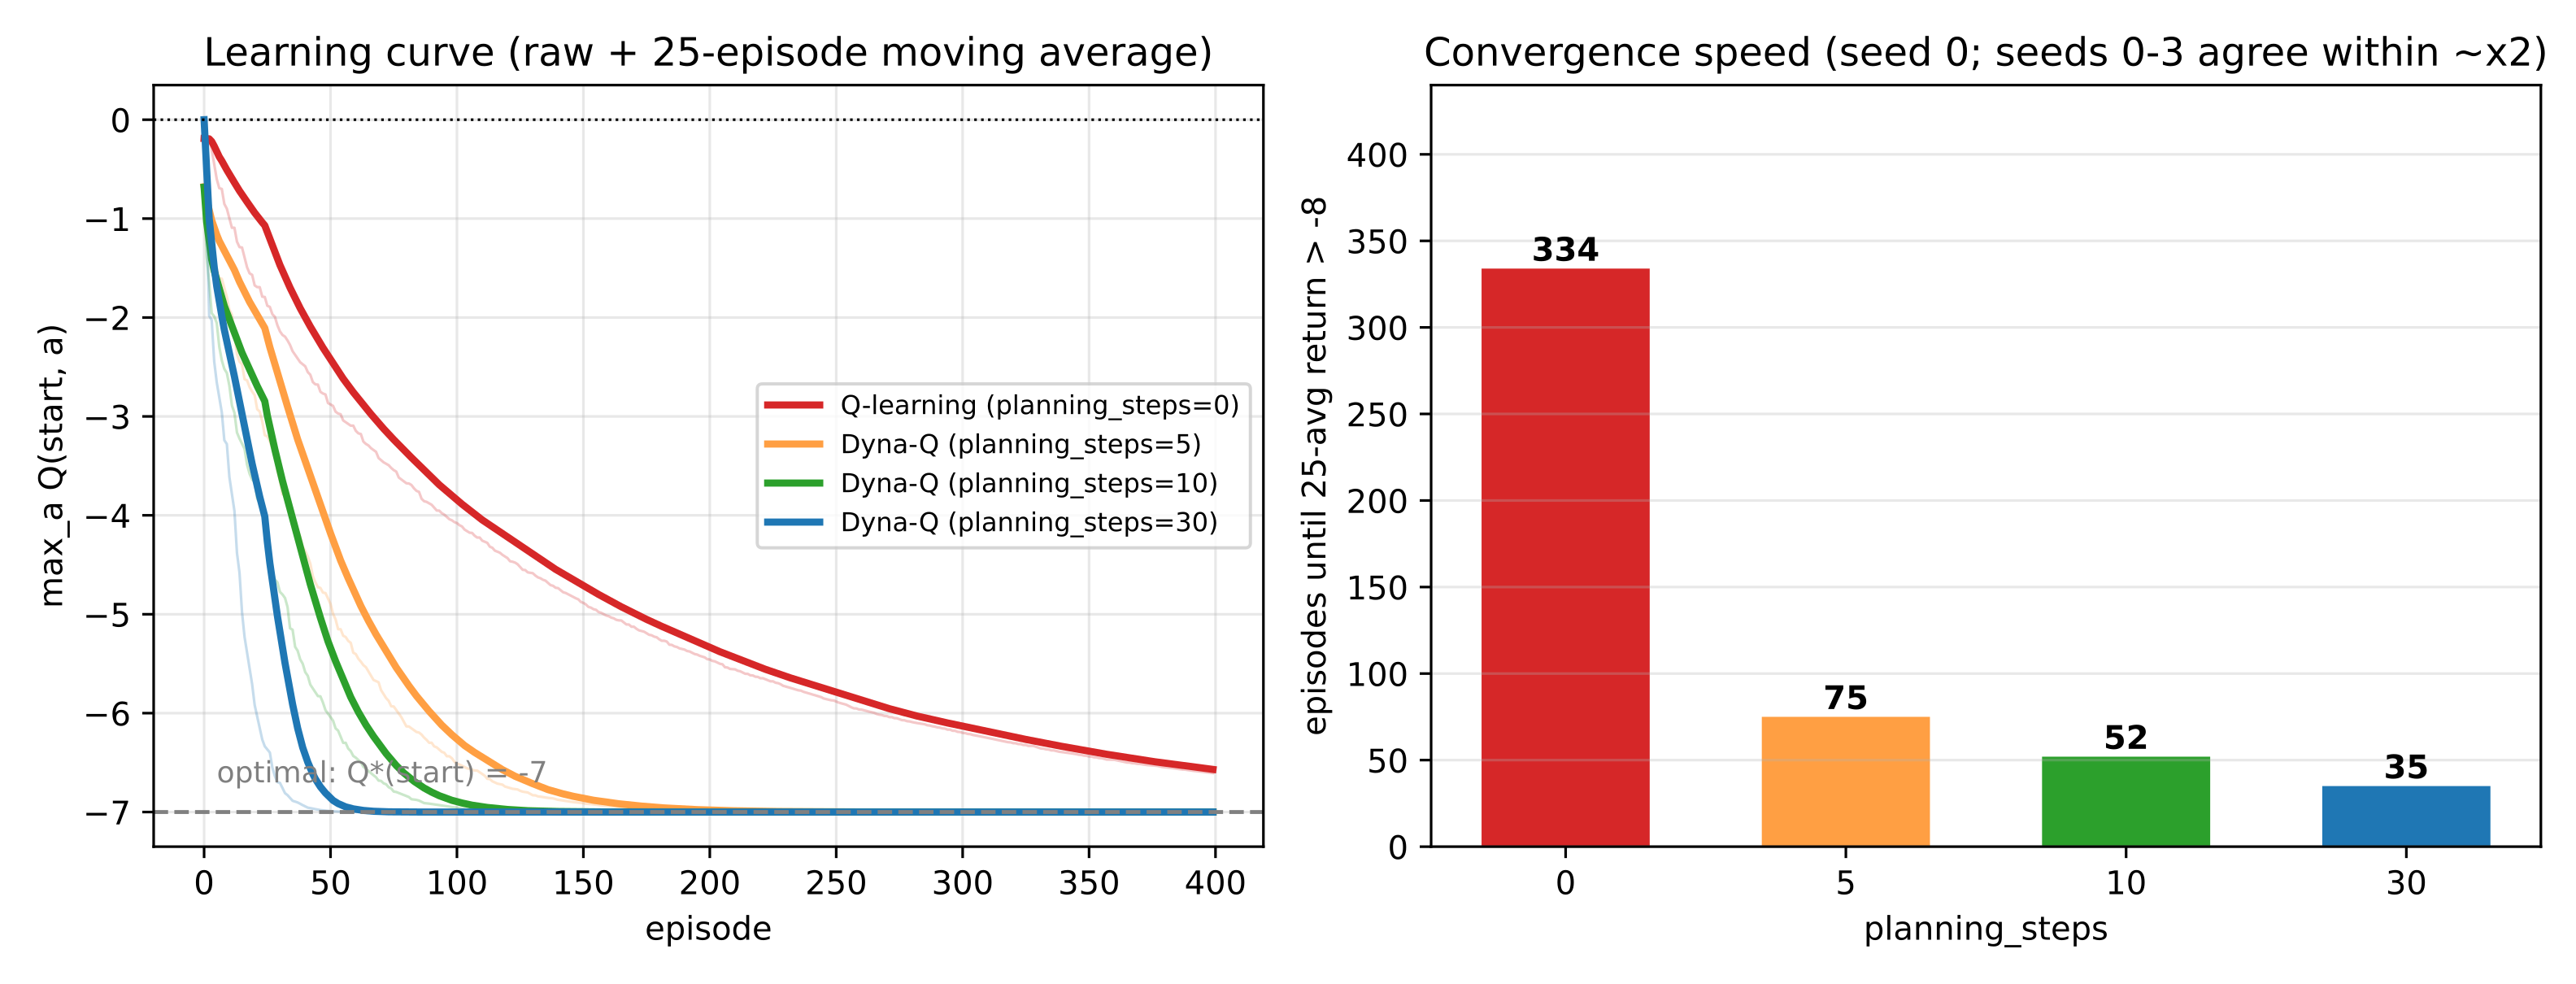
\includegraphics[width=\linewidth]{ch07_3_dyna_q_curves.png}
      {\footnotesize (좌) 매 에피소드 $\max_a Q(\text{출발}, a)$ 학습
      곡선(원본 + 25에피소드 이동평균). 4개 곡선이 참값 $-7$에 접근.
      (우) ``$-8$ 위로 처음 오르는 에피소드'' 막대 그래프 ---
      334(0) $\to$ 35(30), \textbf{약 9.5배} 빠름.}
    \end{column}
    \begin{column}{0.40\textwidth}
      \begin{enumerate}
        \item \textbf{가속은 극적.} 334/35 $\approx$ \textbf{9.5배}.
          실제 상호작용 \textbf{35회}로, 계획 없이는 334회 걸렸던
          학습이 끝.
        \item \textbf{한계 효과 감소.} 0$\to$10: 334$\to$52(약 6배).
          10$\to$30: 52$\to$35(약 1.5배)로만.
        \item \textbf{모델은 거의 포화.} 100개 $(s,a)$ 중 95$\sim$96개
          커버. 작은 격자라 거의 모든 $(s,a)$가 1회 이상 방문 ---
          이 커버리지가 계획 품질의 상한선.
      \end{enumerate}
    \end{column}
  \end{columns}
\end{frame}

\begin{frame}{Dyna-Q 루프 구조도}
  \begin{columns}[T]
    \begin{column}{0.55\textwidth}
      \centering
      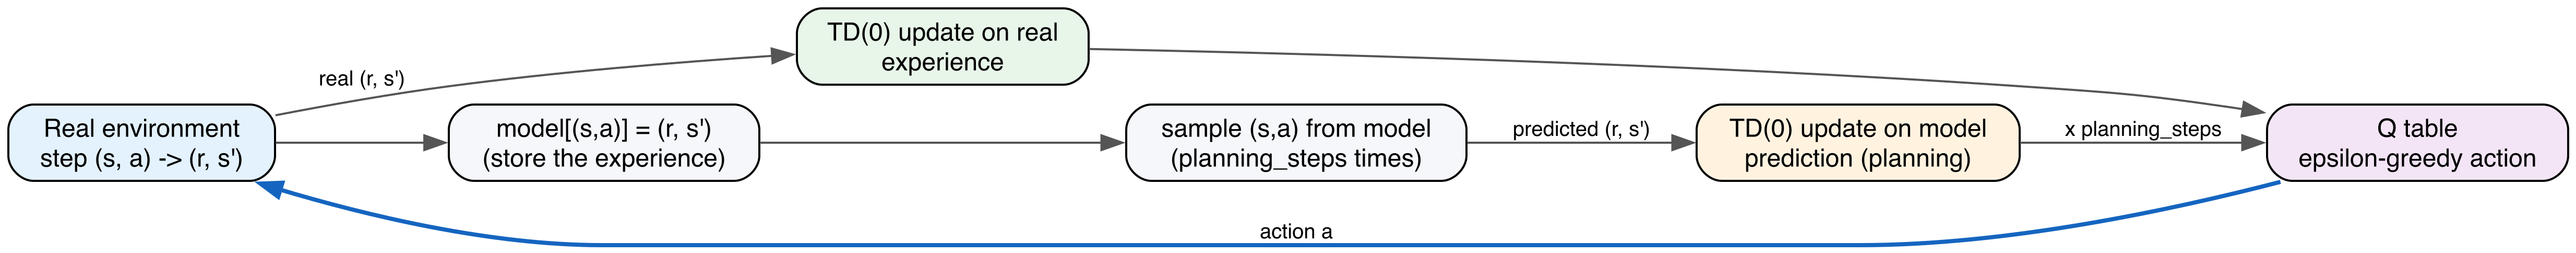
\includegraphics[width=\linewidth]{ch07_3_dyna_q_loop.png}
      {\footnotesize Dyna-Q 루프: (1) 실제 경험으로 TD(0) 갱신,
      (2) \texttt{model[(s,a)] = (r,s')} 저장, (3) 모델에서
      \texttt{planning\_steps}번 무작위 $(s,a)$ 뽑아 가상 TD(0)
      갱신. 실제/계획 갱신 \textbf{모두 하나의 $Q$ 테이블}로 모이고,
      그 $Q$에서 $\varepsilon$-greedy 행동을 뽑아 다시 환경으로.}
    \end{column}
    \begin{column}{0.43\textwidth}
      \begin{block}{왜 \texttt{planning\_steps}이 하이퍼파라미터인지}
        7.2에서 $n$을 ``편향-분산 사이 어딘가''로 튜닝했듯이,
        여기서는 \texttt{planning\_steps}를 \textbf{``계산 비용 대
        가속 효과'' 사이 어딘가}로 튜닝.
        \vskip0.3em
        이번 실험: \textbf{10$\sim$30이 좋은 구간}.
        0(계획 없음)과 ``무한히 크게''(아래 실수 3 참조)는 둘
        다 극단.
      \end{block}
    \end{column}
  \end{columns}
\end{frame}

\begin{frame}{자주 하는 실수 (1/3)}
  \begin{itemize}
    \item \textbf{1. 모델에 없는 $(s,a)$를 직접 조회 $\Rightarrow$
      \texttt{KeyError}.}
      \texttt{model}은 \textbf{희소(sparse) 딕셔너리} --- 아직 한
      번도 경험하지 않은 $(s,a)$는 딕셔너리에 \textbf{그냥
      없음}. \texttt{model[(s,a)]}로 직접 인덱싱하면 처음
      방문하지 않은 상태에서 바로 \texttt{KeyError}.
    \item \textbf{정답}: 계획은 반드시 \texttt{model.items()}에서
      \textbf{이미 있는} $(s,a)$를 무작위로 뽑아야
      (\texttt{random.choice(list(model.items()))}).
    \item ``모델이 아직 불완전하다''는 것은 버그가 아니라
      \textbf{정상 상태} --- 초반엔 모델이 거의 비어 계획이 거의
      아무것도 안 하고, 경험이 쌓일수록 계획 품질도 함께 올라감.
  \end{itemize}
\end{frame}

\begin{frame}{자주 하는 실수 (2/3)}
  \begin{itemize}
    \item \textbf{2. ``실제''와 ``계획''을 \textbf{별도 $Q$ 테이블 두
      개}로 갱신.}
      Dyna-Q가 작동하는 \textbf{전부의 이유}가 \textbf{두 갱신이
      같은 $Q$ 테이블을 공유}하는 것.
    \item 계획만 \texttt{Q\_plan}, 실제 행동만 \texttt{Q\_real}로
      하면, 계획이 만든 값 향상은 \textbf{실제 행동에 한 번도
      반영되지 않음} $\Rightarrow$ 계획을 아무리 많이 돌려도
      실제 학습속도가 1도 안 좋아짐.
    \item \textbf{검증}: 이 절 코드에서 $Q$가 \textbf{하나}이고,
      1번 줄(실제)과 3번 줄(계획)이 \textbf{모두 그 $Q$를
      갱신하는지} 확인.
  \end{itemize}
\end{frame}

\begin{frame}{자주 하는 실수 (3/3)}
  \begin{itemize}
    \item \textbf{3. \texttt{planning\_steps}를 아주 크게 잡기.}
      계획 1회 비용 $\approx$ 실제 스텝 1회 비용.
    \item 그런데 \textbf{모델 오차도 함께 ``복리''로 증식} ---
      모델이 부정확한 초반에 계획을 과도하게 반복하면 그 오차가
      $Q$값에 \textbf{강하게 반영되어 오히려 학습을 방해}.
    \item 단순 계산량으로도 \texttt{planning\_steps=1000}이면
      실제 스텝 1회당 계획 1000회 $\Rightarrow$ \textbf{수렴은
      빨리 안 되면서 만성적으로 느려짐}.
  \end{itemize}
  \vskip0.8em
  \begin{block}{실전}
    \texttt{planning\_steps}도 $\alpha$, $\varepsilon$과
    \textbf{같은 하이퍼파라미터}로, \textbf{검증 성능으로
    튜닝}.
  \end{block}
\end{frame}

\begin{frame}{확인 문제}
  \begin{enumerate}
    \item \kb{공유 테이블.} \texttt{dyna\_q\_grid}에서 계획 갱신(3번
      단계)을 \texttt{Q\_plan} 별도 딕셔너리로 분리하면,
      \texttt{planning\_steps=30}의 수렴 에피소드가 순수
      Q-learning(334)과 어떻게 달라지는지 \textbf{숫자 없이}
      한 문장. (힌트: 계획의 산출물이 어디로 가는가.)
    \item \kb{모델 커버리지.} 400 에피소드 후에도 100개 $(s,a)$ 중
      4개(4\%)가 모델에 안 들어감. 이 ``없는 4개''가 계획에
      미치는 영향을 \texttt{random.choice(list(model.items()))}의
      관점에서 설명.
    \item \kb{참값 판정.} 학습 후 $Q$에서
      $\max(Q[(\text{START}, 0\sim3)]) = -7.00$이고
      $\arg\max$가 ``위''(action 0) 또는 ``오른쪽''(action 3)이면,
      이 정책이 \textbf{최적}인 근거가 손계산 참값(위/오른쪽 $=-7$,
      아래/왼쪽 $=-8$)에 어떻게 대응하는지 설명.
  \end{enumerate}
\end{frame}

\begin{frame}{자주 묻는 질문 (1/2)}
  \begin{itemize}
    \item \kq{Dyna-Q의 모델은 항상 정확한가?}
      --- 학습 초반엔 \textbf{전혀 그렇지 않음}. 몇 번밖에 못
      가본 $(s,a)$쌍의 모델은 부정확하거나 아예 없을 수 있음.
      그런데도 작동하는 이유: 모델이 부정확해도
      \textbf{``그 부정확한 모델로 계획한 결과''가 ``아무것도
      안 하는 것''보다는 대체로 낫고}, 실제 경험이 쌓일수록
      모델도 함께 정확해져 계획 품질도 좋아짐.
    \item \kq{\texttt{planning\_steps}를 무한히 늘리면 항상
      좋아지나?}
      --- 실제 스텝 1회당 계획에 쓰는 계산량이 커질 뿐, 계획
      자체는 \textbf{이미 모은 경험 이상의 새 정보를 만들어내지
      못함}. 모델이 부정확한 상태에서 계획만 과도하게 반복하면
      그 부정확함이 $Q$에 더 강하게 반영 $\Rightarrow$ 오히려
      해로울 수 있음(모델 오차의 ``복리 효과''). 실전:
      \textbf{검증 성능으로 튜닝}.
  \end{itemize}
\end{frame}

\begin{frame}{자주 묻는 질문 (2/2)}
  \begin{itemize}
    \item \kq{Dyna-Q는 on-policy인가, off-policy인가?}
      --- \textbf{off-policy}. $Q$ 갱신 방식은 6.3절 Q-learning과
      \textbf{완전히 같음} --- 목표값에 $\max_a Q(s',a)$(탐욕).
      계획이 모델에서 $(s,a)$를 \textit{무작위}로 뽑는 것은
      ``행동 정책''이 아니라 ``어떤 $(s,a)$의 $Q$를 갱신할지''를
      고르는 것. 갱신 본질엔 여전히 $\max$가 들어감.
    \item \kq{DQN의 경험 재사용(experience replay, Ch.\,9)과
      무엇이 다른가?}
      --- 공통: ``과거 경험을 재사용해 실제 스텝당 갱신을 여러
      번''. 차이: \textbf{재사용의 원천}.
      \begin{itemize}
        \item \textbf{재생}: \textit{실제} $(s,a,r,s')$ 튜플을
          버퍼에서 다시 뽑아 씀 $\Rightarrow$ \textbf{모델 오차
          없음}. 단, 경험한 전이만 재사용할 뿐 \textit{새로운}
          전이는 못 만듦.
        \item \textbf{Dyna-Q 계획}: \textit{모델 예측} $(r,s')$으로
          갱신 $\Rightarrow$ \textbf{모델 오차 동반}. 단, 모델이
          연결한 \textit{아직 경험하지 않은} 상태의 전이까지
          만들 수 있음.
      \end{itemize}
      ``안전하지만 새것을 못 만든다''(재생) vs ``새것을 만들 수
      있지만 오차가 동반된다''(계획) --- 이 트레이드오프가
      Ch.\,9 이후 모델 기반 DQN 변형들의 줄거리.
  \end{itemize}
\end{frame}

\begin{frame}{언제 Dyna-Q가 특히 효과적인가}
  \begin{columns}[T]
    \begin{column}{0.5\textwidth}
      \kb{Dyna-Q가 좋은 상황}
      \begin{itemize}
        \item 실제 상호작용이 \textbf{비싸고}
          (로봇, 물리 실험, 지연 큰 시스템)
        \item 환경이 충분히 \textbf{규칙적}해서
          간단한 모델로 대략 잡아낼 수 있을 때.
      \end{itemize}
    \end{column}
    \begin{column}{0.5\textwidth}
      \kb{모델-프리가 더 좋은 상황}
      \begin{itemize}
        \item 상호작용이 \textbf{아주 싸고}(시뮬레이션, 게임)
        \item 모델 학습이 \textbf{어렵거나}(강한 난수성,
          비마르코프성) 신뢰할 수 없을 때.
      \end{itemize}
    \end{column}
  \end{columns}
  \vskip0.8em
  \begin{block}{첫 번째 판단 기준}
    \kq{``모델을 만들 \textbf{수} 있는가, 만들어도
    \textbf{신뢰}할 만한가''} --- Dyna-Q를 쓸지 말지의
    첫 번째 기준.
  \end{block}
\end{frame}

% ===== wrap-up =====
\begin{frame}{이번 주차 정리}
  \begin{itemize}
    \item \kb{7.1 n-step TD} --- $G_t^{(n)}$은 MC와 TD(0) 사이의
      하나의 다이얼. \texttt{tau = t - n + 1}의 갱신 시차,
      할인 지수 하나만 틀리면 $n=1$이어도 \textbf{편향된 고정점}.
      7-state random walk에서 30 seed 평균 $\Rightarrow$ \textbf{U자}.
      보편적 최적 $n$은 없으므로 검증으로 튜닝.
    \item \kb{7.2 적격흔적} --- 흔적 $e(s)$로 하나의 TD 오차가
      \textbf{모든 상태를 동시에} 후방 갱신. $\lambda$는
      ``$n$ 하나 고르기''를 ``가중치 분포 $\lambda^{n-1}$의
      형태 고르기''로 승화. \textbf{단일 실행은 믿지 말 것}
      (20회 반복 평균). $\lambda=0$ $\Leftrightarrow$ TD(0),
      $\lambda=1$ $\Leftrightarrow$ MC 건성 체크.
    \item \kb{7.3 Dyna-Q} --- 본 $(s,a)$의 $(r,s')$를 모델로
      저장, 실제 스텝마다 모델에서 가상 TD(0) 갱신.
      \textbf{실제/계획이 같은 $Q$ 테이블 공유}가 전부.
      5$\times$5 격자: 334 $\to$ 35 에피소드(약 9.5배),
      한계 효과 + 모델 커버리지가 상한.
  \end{itemize}
  \vskip0.8em
  \begin{block}{다음 주 --- Chapter 8. Block A 캡스톤}
    Gymnasium의 표 기반 환경에서 \textbf{n-step TD · TD($\lambda$) ·
    Dyna-Q를 팀 프로젝트로 직접 구현·비교}. 이번 주 세 다이얼이
    \textbf{같은 질문(``부트스트래핑을 얼마나 할 것인가'')}의
    서로 다른 답이라는 것만 기억하면, 비교 설계가 훨씬 수월해진다.
  \end{block}
\end{frame}

\end{document}
